% !TeX compiler = xelatex
% !TeX encoding = UTF-8

\documentclass[a4paper, 12pt]{article}

% ==========================================
%   1. 基础宏包与字体设置
% ==========================================
\usepackage[UTF8, heading=true]{ctex} % 中文支持
\usepackage{geometry}       % 页面布局
\usepackage{fancyhdr}       % 页眉页脚
\usepackage{graphicx}       % 图片支持
\usepackage{xcolor}         % 颜色支持
\usepackage{tikz}           % 绘图支持
\usetikzlibrary{shadows}    % 【修复】加载 shadows 库以防万一
\usepackage{listings}       % 代码环境
\usepackage[most]{tcolorbox}% 现代盒子
\usepackage{booktabs}       % 专业表格
\usepackage{hyperref}       % 超链接
\usepackage{enumitem}       % 列表定制
\usepackage{float}          % 浮动控制
\usepackage{mathpazo}       % 使用 Palatino 字体
\usepackage{caption}        % 图表标题美化
\usepackage{titletoc}       % 目录美化
\usepackage{multirow}
% ==========================================
%   2. 视觉风格定义
% ==========================================
% --- 颜色定义 ---
\definecolor{ThemeColor}{RGB}{0, 51, 102}    % 主题色：厦大蓝
\definecolor{LightBlue}{RGB}{235, 242, 250}  % 浅蓝背景
\definecolor{CodeBg}{RGB}{250, 250, 250}     % 代码背景：极浅灰
\definecolor{LineNumBg}{RGB}{240, 240, 240}  % 行号背景
\definecolor{CodeGreen}{RGB}{80, 161, 79}    % 代码注释绿
\definecolor{CodePurple}{RGB}{166, 38, 164}  % 代码关键字紫
\definecolor{CodeBlue}{RGB}{64, 120, 242}    % 代码函数蓝

% --- 页面布局 ---
\geometry{left=2.5cm, right=2.5cm, top=3cm, bottom=2.5cm, headheight=25pt}

% --- 链接设置 ---
\hypersetup{
    colorlinks=true,
    linkcolor=ThemeColor,
    filecolor=ThemeColor,      
    urlcolor=ThemeColor,
    pdftitle={操作系统实验报告},
}

% --- 章节标题设置 (ctex) ---
\ctexset{
    section = {
        format = \Large\bfseries\color{ThemeColor},
        beforeskip = 24pt,
        afterskip = 12pt
    },
    subsection = {
        format = \large\bfseries\color{ThemeColor!80!black},
    }
}

% --- 图表标题设置 ---
\DeclareCaptionFont{ThemeColor}{\color{ThemeColor}}
\captionsetup{
    labelfont={bf, ThemeColor},
    textfont={bf},
    labelsep=quad
}

% --- 页眉页脚 ---
\pagestyle{fancy}
\fancyhf{}
\fancyhead[L]{\bfseries\color{ThemeColor} 操作系统实验报告}
\fancyhead[R]{\small\leftmark}
\fancyfoot[C]{\thepage}
\renewcommand{\headrulewidth}{1pt}
\renewcommand{\headrule}{\hbox to\headwidth{\color{ThemeColor}\leaders\hrule height \headrulewidth\hfill}}

% --- 目录样式美化 ---
\titlecontents{section}[0pt]{\addvspace{10pt}\bfseries}
{\color{ThemeColor}\thecontentslabel\hspace{1em}}
{}
{\titlerule*[8pt]{.}\contentspage}

\titlecontents{subsection}[2em]{\addvspace{3pt}}
{\thecontentslabel\hspace{1em}}
{}
{\titlerule*[8pt]{.}\contentspage}


\newtcblisting{codeblock}[2][]{%
	enhanced, breakable, listing engine=listings, listing only,%
	title={#2}, coltitle=black!80, fonttitle=\footnotesize\bfseries\sffamily,%
	attach boxed title to top left={xshift=22mm, yshift=-3.5mm},%
	boxed title style={empty, size=minimal, bottom=0pt, top=0pt},%
	colback=CodeBg, colframe=gray!25, boxrule=0.5pt, arc=4mm,%
	left=6mm, right=4mm, top=10mm, bottom=4mm,%
	drop shadow={opacity=0.15},%
	underlay={%
		\begin{tcbclipinterior}
			\fill[gray!5] (frame.north west) rectangle ([yshift=-9mm]frame.north east);
			\fill[LineNumBg] (frame.south west) rectangle ([xshift=5.5mm]frame.north west);
		\end{tcbclipinterior}%
	},%
	overlay={%
		\draw[fill=red!60, draw=red!70] ([xshift=6mm, yshift=-4.5mm]frame.north west) circle (2pt);
		\draw[fill=orange!60, draw=orange!70] ([xshift=11mm, yshift=-4.5mm]frame.north west) circle (2pt);
		\draw[fill=green!60!black!60, draw=green!60!black!70] ([xshift=16mm, yshift=-4.5mm]frame.north west) circle (2pt);
	},%
	listing options={%
		language=C, basicstyle=\ttfamily\footnotesize, keywordstyle=\color{CodePurple}\bfseries,%
		commentstyle=\color{CodeGreen}\itshape, stringstyle=\color{orange!80!black},%
		ndkeywordstyle=\color{CodeBlue}\bfseries, numbers=left, numberstyle=\tiny\color{gray!60}\ttfamily,%
		stepnumber=1, numbersep=10pt, breaklines=true, tabsize=4, showstringspaces=false,%
		frame=none, escapeinside={(*@}{@*)}, columns=fixed, keepspaces=true%
	},%
	#1%
}

% 图片占位宏 (修复版)
\newcommand{\placeholderimg}[3]{
    \begin{figure}[H]
        \centering
        \begin{tikzpicture}
            % 如果没有 logo 图片，请注释掉下面这一行
            \node[opacity=0.1] {
\includegraphics[width=3cm]{img/logo.png}}; 
            \node[align=center] at (0,0) {
                \color{ThemeColor}\bfseries\Large 图片占位符 \\[1em]
                \color{gray}\small 尺寸: #1 $\times$ #2 \\[0.5em]
                \color{black}\itshape #3
            };
        \end{tikzpicture}
        % 【修复点2】移除了自动生成的 label，避免复杂字符报错
        \caption{#3} 
    \end{figure}
}

% ==========================================
%   4. 文档正文
% ==========================================
\begin{document}
    
    % --- 封面 ---
    \begin{titlepage}
        \newgeometry{top=3cm, bottom=2cm, left=2cm, right=2cm}
        \centering
        
        % 顶部装饰
        \begin{tikzpicture}[remember picture, overlay]
            \fill[ThemeColor] (current page.north west) rectangle ([yshift=-1cm]current page.north east);
        \end{tikzpicture}
        
        \vspace*{1cm}
        % Logo (确保 img/logo.png 存在，否则替换为文件名或注释掉)
        
\includegraphics[width=8cm]{img/logo.png} 
        
        \vspace{1cm}
        
        {\Huge \bfseries \heiti 操作系统实验报告 \par}
        \vspace{0.5cm}
        {\color{ThemeColor} \rule{0.6\textwidth}{1.5pt}} % 分割线
        \vspace{0.5cm}
        
        {\Large \bfseries 实验三：调度算法比较 \par}
        
        \vspace{1.5cm}
        
        % 信息表格
        \begin{large}
            \renewcommand{\arraystretch}{2.0}
            \begin{tabular}{rc}
                \bfseries 专\hspace{1em}业： & \underline{\makebox[8cm][c]{人工智能}} \\
                \bfseries 姓\hspace{1em}名： & \underline{\makebox[8cm][c]{张晓宇}} \\
                \bfseries 学\hspace{1em}号： & \underline{\makebox[8cm][c]{37220232203927}} \\
                \bfseries 实验日期： & \underline{\makebox[8cm][c]{2025.12.5}} \\
                \bfseries 指导教师： & \underline{\makebox[8cm][c]{曹冬林}} \\
            \end{tabular}
        \end{large}
        
        \vfill
        {\small \today}
    \end{titlepage}
    \restoregeometry
    
    % --- 目录 ---
    {
        \hypersetup{linkcolor=black} 
        \tableofcontents
    }
    \newpage
    
    % --- 正文 ---
    
    \section{实验目的}
    
    本次实验围绕操作系统的核心主题——进程调度算法展开，旨在达成以下目标：
    
    \subsection{深入理解进程调度机制}
    学习操作系统中进程调度器的工作原理，理解调度器如何在多个就绪进程之间进行选择。掌握调度策略与调度算法的区别，以及不同调度算法对系统性能的影响。
    
    \subsection{掌握多种调度算法的原理与实现}
    研究并实现四种经典的进程调度算法：
    \begin{itemize}[label=\textbullet, itemsep=0pt]
        \item \textbf{优先级调度（Priority Scheduling）}：根据进程优先级选择执行，优先级高的进程优先获得CPU。
        \item \textbf{先来先服务（FCFS）}：按照进程到达就绪队列的先后顺序进行调度。
        \item \textbf{轮转调度（Round Robin）}：进程按照循环顺序轮流获得时间片执行。
        \item \textbf{静态多级队列（SML）}：将进程按优先级划分到不同队列，高优先级队列优先调度，队列内部使用轮转策略。
    \end{itemize}
    
    \subsection{设计调度算法评估框架}
    构建一个可切换的调度框架，支持在运行时动态切换调度算法。设计合理的测试方案，包含不同类型的负载（CPU密集型和IO密集型），对调度算法进行公平的性能对比。
    
    \subsection{掌握调度算法性能分析方法}
    学习进程运行时间统计方法，理解就绪时间、运行时间、休眠时间、周转时间等关键指标的含义。通过对比实验，分析不同调度算法在各项指标上的表现差异。
    
    \section{实验环境}
    
    \subsection{硬件环境}
    \begin{itemize}[label=\textbullet, itemsep=0pt]
        \item \textbf{CPU}：Intel i9-13900h
        \item \textbf{GPU}：NVIDIA RTX 4050
        \item \textbf{宿主机操作系统}：Windows 11
    \end{itemize}
    
    \subsection{软件环境}
    \begin{itemize}[label=\textbullet, itemsep=0pt]
        \item \textbf{操作系统}：Ubuntu 18.04 (64位)
        \item \textbf{模拟器}：QEMU
        \item \textbf{编译工具}：gcc, make (build-essential)
        \item \textbf{目标操作系统内核}：xv6
    \end{itemize}
    
    \section{实验要求}
    
    \subsection{任务一：实现调度算法}
    在 \texttt{proc.c} 中编程实现以下四种调度算法：
    \begin{enumerate}
        \item \textbf{优先级调度（Priority Scheduling）}：选择优先级最高（数值最小）的就绪进程执行。
        \item \textbf{先来先服务（FCFS）}：选择创建时间最早的就绪进程执行。
        \item \textbf{轮转调度（Round Robin）}：按循环顺序公平地调度每个就绪进程。
        \item \textbf{静态多级队列（SML）}：按优先级将进程划分为多个队列，高优先级队列优先执行。
    \end{enumerate}
    
    \subsection{任务二：实现测试程序}
    在 \texttt{scheduler\_test.c} 中实现测试程序：
    \begin{enumerate}
        \item 创建 6 个进程，包含 3 个 CPU 密集型进程和 3 个 IO 密集型进程。
        \item 为不同类型的进程设置不同的优先级。
        \item 记录所有进程的运行过程，收集进程统计信息。
        \item 对比各调度算法在平均就绪时间、平均运行时间、平均休眠时间、平均周转时间上的结果。
    \end{enumerate}
    
    \section{实验流程}
    
    实验三完成思路流程图如下：
    
       	\begin{figure}[H] 
    	\centering
    	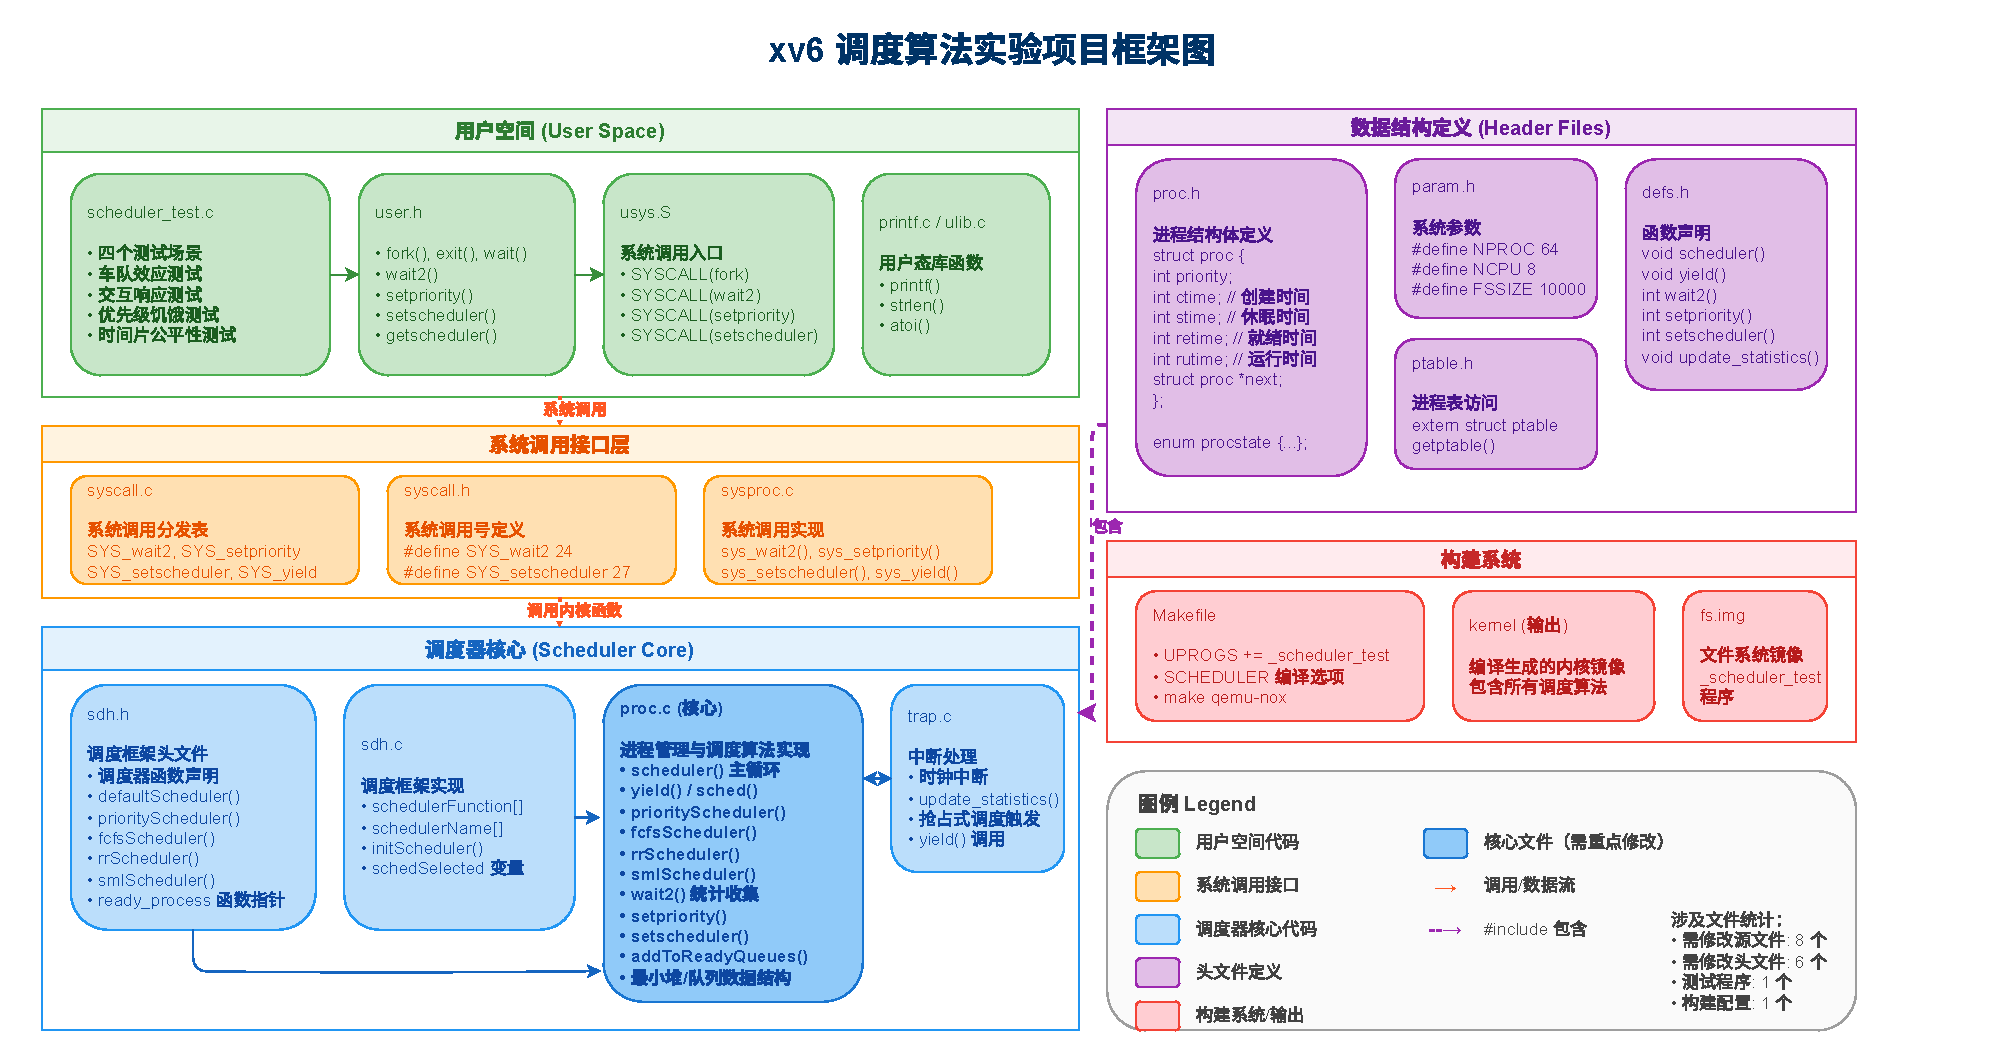
\includegraphics[width=1.0\textwidth]{img3/project_framework.drawio.pdf}
    	\caption{本项目总体框架}
    	\label{fig:code_framework}
    \end{figure}
        
    \begin{figure}[H] 
	        \centering
	        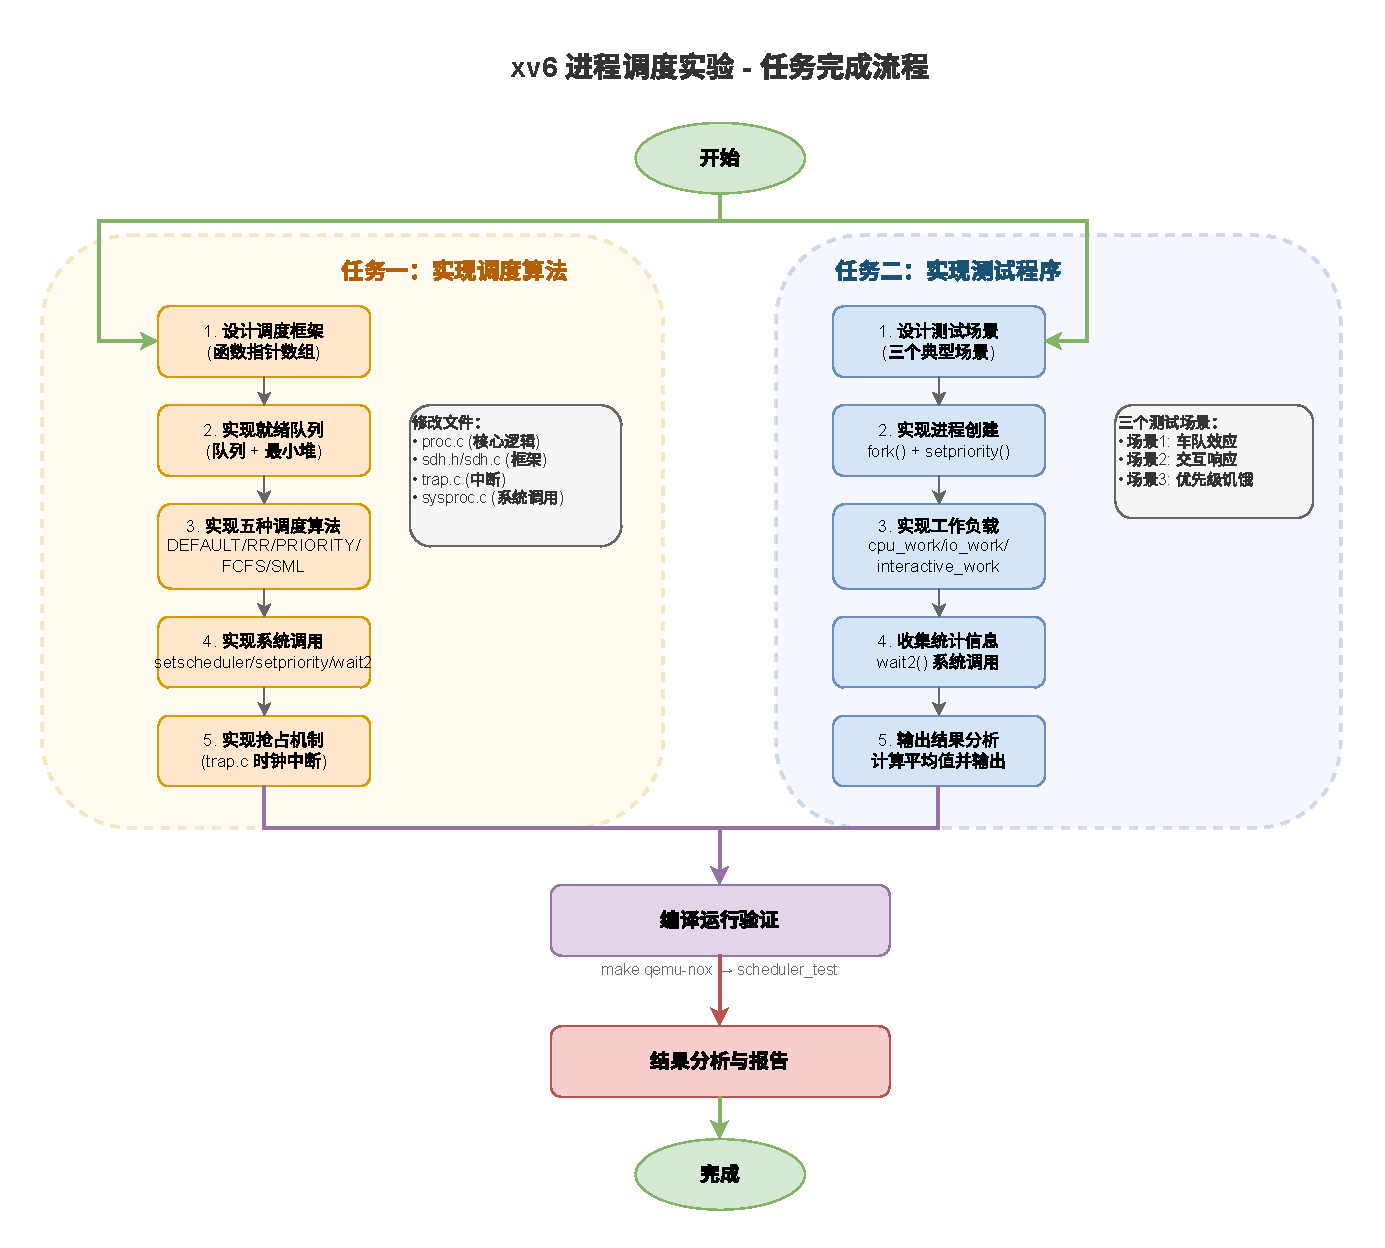
\includegraphics[width=1.0\textwidth]{img/experiment_workflow.drawio.pdf}
	        \caption{实验完成流程}
	        \label{fig:scheduler_selection}
   	\end{figure}
    
    \subsection{实验准备：调度框架设计}
    本次实验需要设计一个可扩展的调度框架，支持在运行时动态切换调度算法。同时需要扩展进程控制块以支持运行时间统计。
    
    \subsubsection{扩展进程控制块}
    为了支持调度算法比较，需要在 \texttt{proc.h} 的进程控制块中添加以下时间统计字段：
    \begin{itemize}
        \item \texttt{priority}：进程优先级 (1-20)
        \item \texttt{ctime}：进程创建时间
        \item \texttt{stime}：休眠(SLEEPING)累计时间
        \item \texttt{retime}：就绪(RUNNABLE)累计时间
        \item \texttt{rutime}：运行(RUNNING)累计时间
    \end{itemize}
    
    \subsubsection{调度框架设计}
    在 \texttt{sdh.h} 中设计可扩展的调度框架，核心思想是使用函数指针数组存储各调度算法，通过 \texttt{setscheduler()} 系统调用动态切换当前使用的调度函数。
    
    调度框架的设计思路如图\ref{fig:scheduler_selection}所示。
    
    \subsubsection{就绪队列实现}
    
    为了提高调度效率，实现了真正的就绪队列数据结构。
    
    \textbf{队列与堆结构设计：}
    
    在 \texttt{proc.c} 中定义了不同的数据结构支持各种调度算法：
    \begin{itemize}
        \item \texttt{fcfsQueue}：用于 FCFS 和 RR 调度的先进先出队列（1个队列）
        \item \texttt{pHeap}：用于优先级调度的\textbf{最小堆}结构，时间复杂度 O(log n)
        \item \texttt{smlQueues[3]}：用于静态多级队列调度（3个队列：高/中/低）
    \end{itemize}
    
    \textbf{最小堆优化说明：}
    
    优先级调度采用最小堆而非多级队列实现，具有以下优势：
    \begin{itemize}
        \item 插入进程：O(log n)，通过 \texttt{siftUp()} 上浮操作维护堆性质
        \item 提取最高优先级进程：O(log n)，通过 \texttt{siftDown()} 下沉操作
        \item 堆的性质：父节点优先级 $\leq$ 子节点优先级（数值越小优先级越高）
    \end{itemize}
    
    \textbf{核心实现：}
    
    \begin{codeblock}{enqueue}
    // 入队：将进程添加到队列尾部
        void enqueue(struct procqueue *q, struct proc *p) {
        p->next = 0;
        if (q->tail == 0) {
            q->head = q->tail = p;
        } else {
            q->tail->next = p;
            q->tail = p;
        }
        }
    \end{codeblock}
    
    \begin{codeblock}{dequeue}
// 出队：从队列头部取出进程
struct proc *dequeue(struct procqueue *q) {
    struct proc *p = q->head;
    if (p == 0)
    return 0;
    q->head = p->next;
    if (q->head == 0) {
    q->tail = 0;
    }
    p->next = 0;
    return p;
}
    \end{codeblock}
    
        \begin{codeblock}{addToReadyQueues}
        
        // 统一入队函数：进程变为 RUNNABLE 时调用
        // 根据当前激活的调度器，只添加到对应的队列
        extern int schedSelected; // 来自 sdh.h，表示当前调度器类型
        
        void addToReadyQueues(struct proc *p) { // 将进程p加入到就绪队列
        switch (schedSelected) {
            case 0: // DEFAULT - 使用 fcfsQueue
            case 2: // FCFS
            case 3: // RR (CFS)
            enqueue(\&fcfsQueue, p);
            break;
            case 1: // PRIORITY - 使用最小堆
            heapInsert(p);
            break;
            case 4: // SML
            if (p->priority >= 1 \&\& p->priority <= 7) {
            enqueue(\&smlQueues[0], p);
            } else if (p->priority >= 8 \&\& p->priority <= 14) {
            enqueue(\&smlQueues[1], p);
            } else {
            enqueue(\&smlQueues[2], p);
            }
            break;
            default:
            enqueue(\&fcfsQueue, p);
            break;
        }
        }
    \end{codeblock}
    \textbf{调度器选择机制：}
    
    调度器选择通过编译时宏定义和运行时函数指针两种机制实现：
    \begin{enumerate}
        \item \textbf{编译时}：通过 Makefile 传递 \texttt{SCHEDPOLICY} 宏，在 \texttt{sdh.h} 中初始化 \texttt{ready\_process} 函数指针
        \item \textbf{运行时}：通过 \texttt{setscheduler(sid)} 系统调用动态切换调度器，同时重建就绪队列
    \end{enumerate}
    
    调度器选择机制流程如图\ref{fig:sched_framework}所示。
    
    \begin{figure}[H] 
    	\centering
    	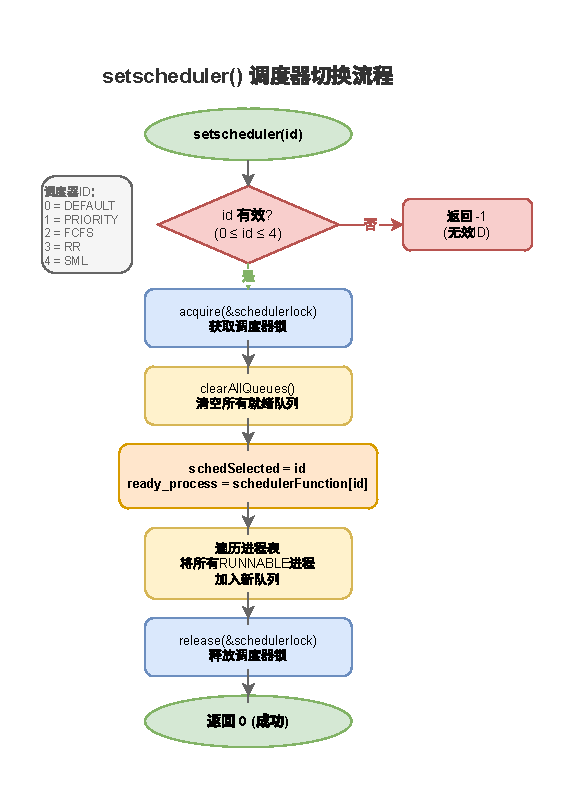
\includegraphics[width=0.7\textwidth]{img/setscheduler.drawio.pdf}
    	\caption{调度器选择框架设计流程}
    	\label{fig:sched_framework}
    \end{figure}
    
    
%    \begin{figure}[H] 
%        \centering
%        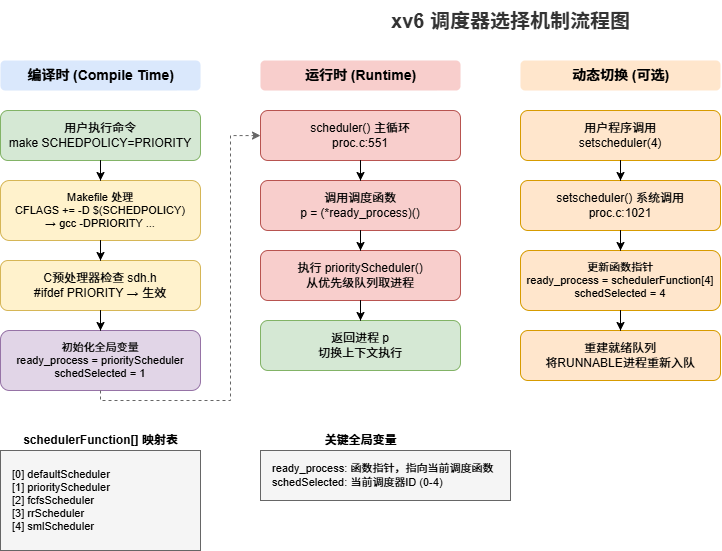
\includegraphics[width=0.9\textwidth]{img/scheduler_selection_flow.png}
%        \caption{调度器选择机制流程}
%        \label{fig:scheduler_selection}
%    \end{figure}
    
    \subsubsection{进程统计信息收集}
    实现 \texttt{update\_statistics()} 函数，在每个时钟中断时被调用，根据当前进程状态更新对应的时间计数器。该函数遍历进程表，根据进程的 SLEEPING、RUNNABLE、RUNNING 状态分别递增 \texttt{stime}、\texttt{retime}、\texttt{rutime} 计数器。
    
    \subsection{任务一：实现调度算法}
    
    \subsubsection{调度器主循环}
    修改 \texttt{scheduler()} 函数，使用函数指针 \texttt{ready\_process} 调用当前选择的调度算法，实现调度策略的动态切换。
    
   \textbf{ 调度器函数：}
    
    \begin{codeblock}{scheduler}
    // scheduler - 调度器主循环函数
    // 功能：操作系统的核心调度循环，负责选择并切换到下一个要执行的进程
    // 说明：此函数永不返回，每个CPU核心启动后会一直在此循环中运行
    void scheduler(void) {
    struct proc *p;          // 指向被选中进程的指针
    struct cpu *c = mycpu(); // 获取当前CPU结构体
    c->proc = 0;             // 初始化：当前CPU没有运行任何进程
    
    for (;;) { // 无限循环：调度器永不停止
        // 步骤1：启用中断
        sti(); // SeT Interrupt flag（设置中断标志）主要目的：
        // 若无就绪进程，CPU会空转，设置中断标志后时钟中断可以触发，从而调用wakeup()。否则会死锁
        
        // 步骤2：获取进程表锁，准备查找就绪进程
        acquire(\&ptable.lock);
        
        // 步骤3：调用当前选定的调度算法选择下一个进程
        acquire(\&schedulerlock);
        p = (*ready_process)(); // 调用调度算法函数（如priorityScheduler、fcfsScheduler等）
        release(\&schedulerlock);
        
        // 步骤4：如果找到了就绪进程，则进行上下文切换
        if (p != 0) {
        // 4.1 设置当前CPU正在运行的进程
        c->proc = p;
        
        // 4.2 切换到进程的页表（用户地址空间）
        switchuvm(p);
        
        // 4.3 将进程状态标记为RUNNING
        p->state = RUNNING;
        
        // 4.4 执行上下文切换：保存调度器上下文，恢复进程上下文
        swtch(\&(c->scheduler), p->context);
        
        // 4.5 进程p切换回来后，恢复内核页表
        switchkvm();
        
        // 4.6 清理：当前CPU不再运行任何进程
        c->proc = 0;
        }
        
        // 步骤5：释放进程表锁
        release(\&ptable.lock);
    }
    }
    \end{codeblock}
    
    调度器主循环流程如图\ref{fig:scheduler_main}所示。
    
    \begin{figure}[H] 
        \centering
        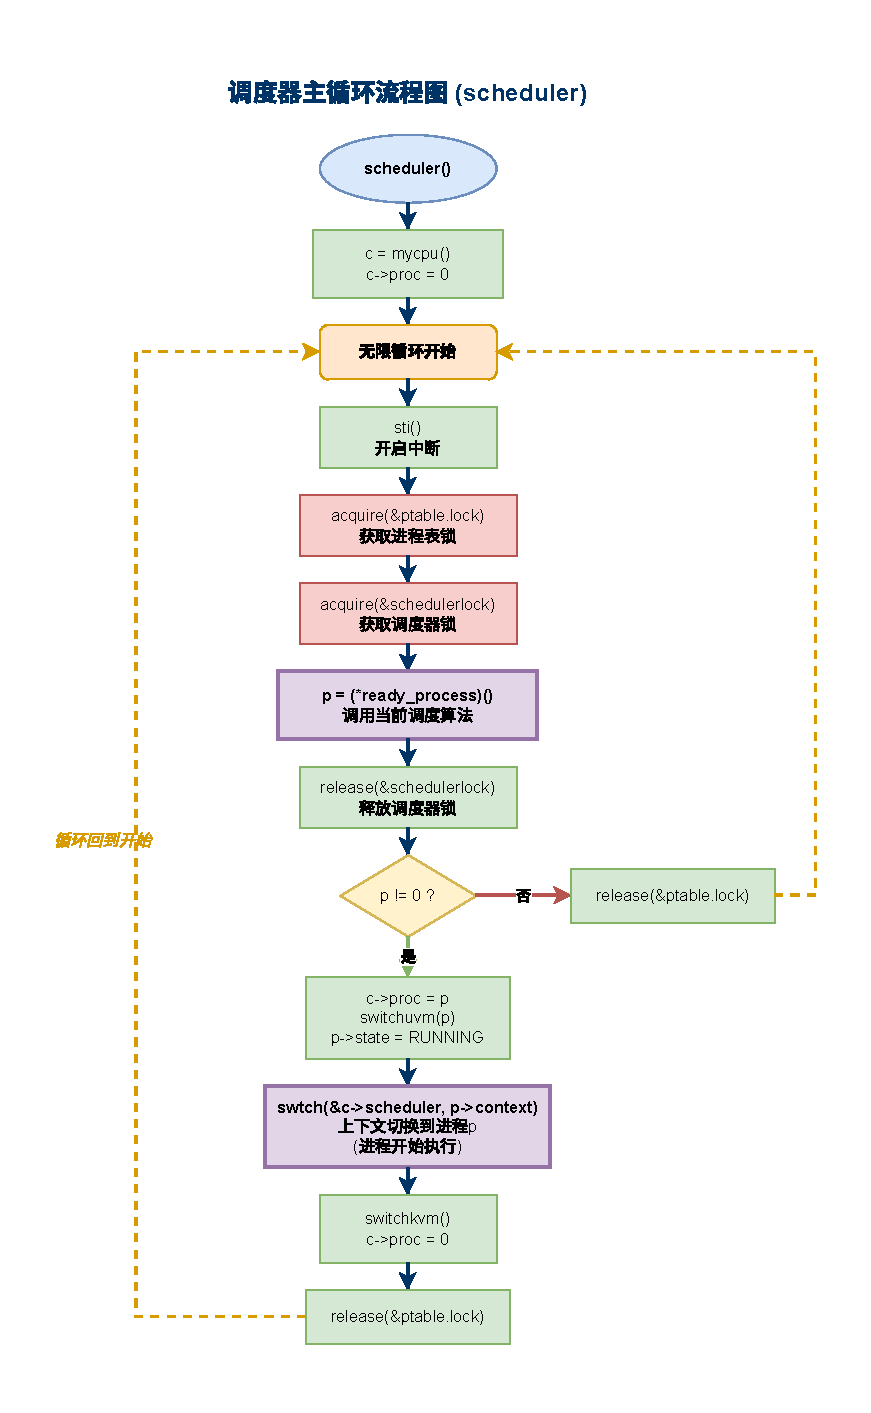
\includegraphics[width=0.8\textwidth]{img/scheduler_main.drawio.pdf}
        \caption{调度器主循环流程}
        \label{fig:scheduler_main}
    \end{figure}
    
    \subsubsection{优先级调度算法（Priority Scheduling）}
    
    \textbf{算法原理：}
    
    优先级调度是一种基于进程重要性的抢占式或非抢占式调度算法。每个进程被分配一个优先级值，调度器总是选择优先级最高的就绪进程执行。在本实现中，优先级使用数值1-20表示，\textbf{数值越小表示优先级越高}。
    
    该算法的核心思想是：\textit{重要的任务应该优先得到CPU资源}。通过为不同类型的进程分配不同的优先级，系统可以确保关键任务（如系统服务、实时任务）能够快速响应，而次要任务（如后台批处理）则在资源空闲时执行。
    
    \textbf{实现策略：}
    
    本实现采用\textbf{最小堆}数据结构实现非抢占式优先级调度，具体设计如下：
    \begin{enumerate}[itemsep=2pt]
        \item 使用结构体 \texttt{priorityHeap} 存储就绪进程指针数组和堆大小
        \item 插入时调用 \texttt{heapInsert()}，将进程放入堆末尾后执行 \texttt{siftUp()} 上浮
        \item 提取时调用 \texttt{heapExtract()}，取出堆顶后将末尾元素放到堆顶，执行 \texttt{siftDown()} 下沉
        \item 堆顶始终是优先级最高（数值最小）的进程
    \end{enumerate}
    
    相比遍历进程表的 O(n) 实现，最小堆将提取操作优化到 O(log n)。
    \begin{enumerate}[itemsep=2pt]
        \item 遍历整个进程表，筛选出所有状态为 RUNNABLE 的就绪进程
        \item 维护一个候选进程指针 \texttt{highP}，初始值为 NULL
        \item 对每个就绪进程，比较其 \texttt{priority} 字段与当前候选进程
        \item 如果发现更高优先级的进程（数值更小），则更新候选进程指针
        \item 遍历完成后，返回优先级最高的进程
    \end{enumerate}
    
    \textbf{算法优势：}
    \begin{itemize}[itemsep=0pt]
        \item \textbf{响应快速}：高优先级进程可以立即获得CPU，适合实时系统
        \item \textbf{灵活性高}：可以根据实际需求动态调整进程优先级
        \item \textbf{实现简单}：只需一次遍历即可完成调度决策
    \end{itemize}
    
    \textbf{潜在问题：}
    \begin{itemize}[itemsep=0pt]
        \item \textbf{饥饿问题}：低优先级进程可能永远得不到执行机会
        \item \textbf{不够公平}：相同优先级的进程之间没有轮转机制
    \end{itemize}
    
    优先级调度算法的实现流程如图\ref{fig:priority_sched}所示。
    
%    \begin{figure}[H] 
%        \centering
%        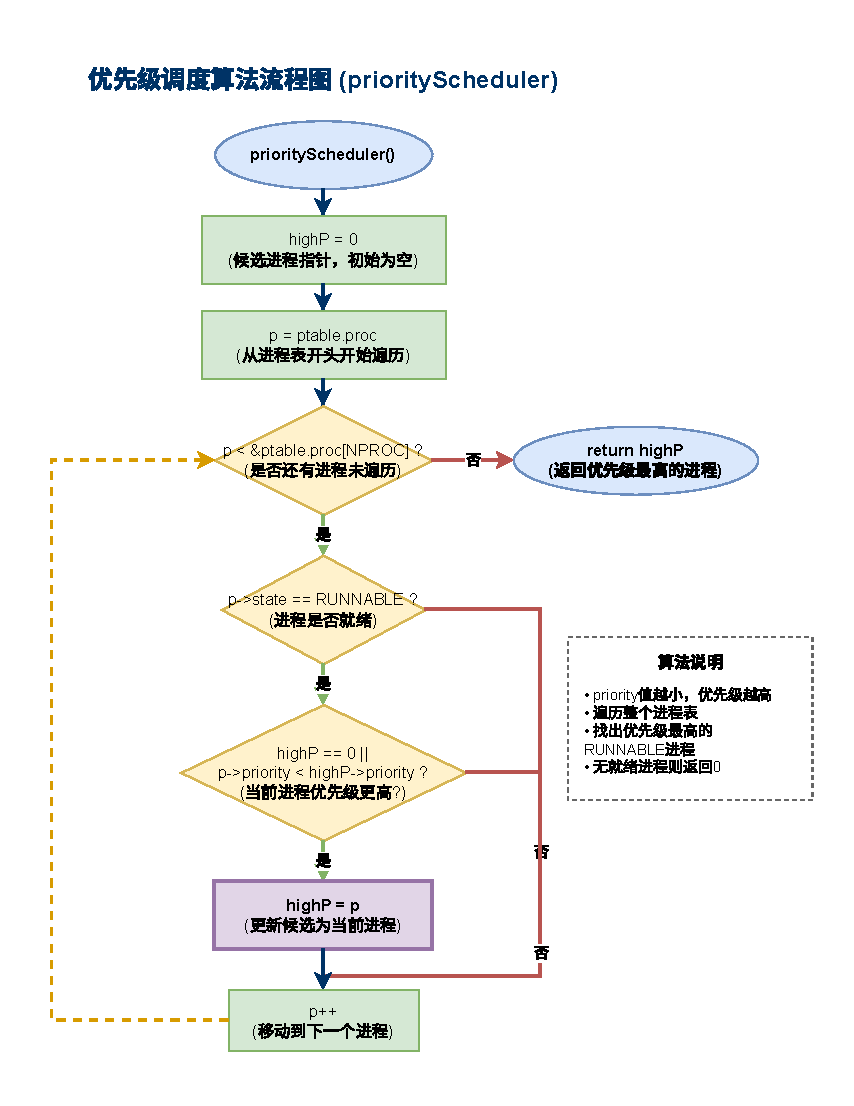
\includegraphics[width=0.7\textwidth]{img/priority_scheduler.drawio.pdf}
%        \caption{优先级调度算法实现流程}
%        \label{fig:priority_sched}
%    \end{figure}
    
    \textbf{核心代码实现：}
    
    优先级调度算法的核心代码如下。
    \begin{codeblock}{priorityScheduler}
        // Priority Scheduler -------------------
        // 使用最小堆提取优先级最高（数值最小）的 RUNNABLE 进程
        // 时间复杂度 O(log n)
        struct proc *priorityScheduler() {
        return heapExtract();  // 从最小堆中提取堆顶（优先级最高的进程）
        }
    \end{codeblock}

    
    \subsubsection{先来先服务调度算法（FCFS）}
    
    \textbf{算法原理：}
    
    先来先服务（First-Come First-Served）是最简单直观的调度算法，遵循"先到先得"的公平原则。进程按照进入就绪队列的时间顺序排队，调度器总是选择最早到达的进程执行，直到该进程执行完毕或主动放弃CPU。
   
    
    \textbf{实现策略：}
    
    \begin{codeblock}{fcfsScheduler}
        // FCFS Scheduler -----------------------
        struct proc *fcfsScheduler() { // 先来先服务
        return dequeue(\&fcfsQueue);  // 从就绪顺序队列中取出
        }
    \end{codeblock}
    
    
    \textbf{算法优势：}
    \begin{itemize}[itemsep=0pt]
        \item \textbf{实现简单}：无需复杂的数据结构和调度决策逻辑
        \item \textbf{公平性好}：所有进程按到达顺序依次执行，不会饥饿
        \item \textbf{可预测性强}：进程等待时间可以根据队列长度估算
    \end{itemize}
    
    \textbf{潜在问题：}
    \begin{itemize}[itemsep=0pt]
        \item \textbf{护航效应（Convoy Effect）}：一个长进程会阻塞后面所有短进程
        \item \textbf{平均等待时间长}：短作业可能因为前面的长作业而等待很久
        \item \textbf{不适合交互式系统}：无法优先响应用户交互请求
    \end{itemize}
    
    FCFS 调度算法原理如图\ref{fig:FIFS}所示。
    
    \begin{figure}[H] 
        \centering
        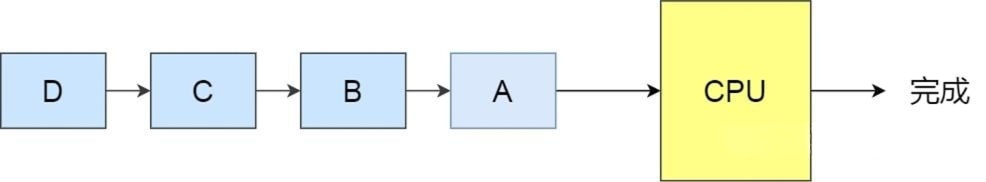
\includegraphics[width=0.85\textwidth]{img/FIFS.jpeg}
        \caption{先来先服务调度原理}
        \label{fig:FIFS}
    \end{figure}
    
    
    \subsubsection{轮转调度算法（Round Robin）}
    
    \textbf{算法原理：}
    
    轮转调度（Round Robin，简称RR）是一种\textbf{时间片轮转}的抢占式调度算法，被广泛应用于分时操作系统中。其核心思想是：将CPU时间划分为固定长度的时间片（time quantum），就绪队列中的进程按\textbf{循环顺序}依次获得一个时间片的执行机会。
    
    当一个进程的时间片用完后，即使它尚未完成，也会被迫让出CPU，回到就绪队列末尾等待下一轮调度。这种机制保证了所有进程都能\textit{公平地}获得CPU资源，不会出现某个进程长期占用CPU的情况。
    
    \textbf{实现策略：}
    
    \begin{codeblock}{rrScheduler}
        // Round Robin Scheduler -------------------------
        struct proc *rrScheduler() {  // 轮转调度
        return dequeue(\&fcfsQueue); // 从FCFS队列取出，调度后由yield重新入队尾
        // 当前文件中与先来先服务的实现相同，但是在trap.c中，只有轮转是抢占式，即只有轮转会被时钟中断抢占
        }
    \end{codeblock}
    
    \textbf{时间片设置：}在xv6中，时间片由时钟中断频率决定，默认为10ms。\textbf{只有 RR 调度器}在时钟中断时会强制调用 \texttt{yield()} 让出CPU，其他调度器（FCFS、PRIORITY、SML）均为非抢占式。
    
    \textbf{算法优势：}
    \begin{itemize}[itemsep=0pt]
        \item \textbf{公平性极佳}：所有进程获得相同的CPU时间配额
        \item \textbf{响应时间好}：交互式任务不会等待太久
        \item \textbf{无饥饿问题}：每个进程都保证在有限时间内得到调度
        \item \textbf{适合分时系统}：特别适合多用户、多任务环境
    \end{itemize}
    
    \textbf{潜在问题：}
    \begin{itemize}[itemsep=0pt]
        \item \textbf{上下文切换开销}：频繁切换进程会增加系统开销
        \item \textbf{时间片难以选择}：过长影响响应时间，过短增加开销
        \item \textbf{不区分优先级}：无法优先服务重要进程
    \end{itemize}
    
    轮转调度算法原理如图\ref{fig:RR}所示。
    
    \begin{figure}[H] 
        \centering
        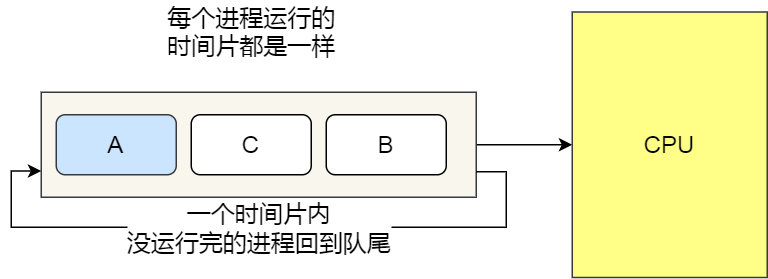
\includegraphics[width=0.7\textwidth]{img/RoundRobin.jpg}
        \caption{轮转调度原理}
        \label{fig:RR}
    \end{figure}
    
    
    \subsubsection{静态多级队列调度算法（SML）}
    
    \textbf{算法原理：}
    
    静态多级队列（Static Multi-Level Queue）是一种\textbf{混合型调度算法}，它巧妙地结合了优先级调度和轮转调度的优点。该算法的核心思想是：根据进程的优先级将其\textit{永久性地}分配到不同的就绪队列中，高优先级队列总是优先得到调度，而队列内部则采用轮转策略保证公平性。
    
    "静态"体现在进程一旦被分配到某个队列，其所属队列关系就固定不变；"多级"则体现在系统维护多个不同优先级的就绪队列。这种设计既保证了重要进程的响应速度，又避免了同等重要进程之间的不公平竞争。
    
    \textbf{队列划分策略：}
    
    本实现将进程按优先级划分为三个队列：
    \begin{itemize}[itemsep=2pt]
        \item \textbf{队列1（高优先级）}：priority 1-7 \quad （系统服务、实时任务）
        \item \textbf{队列2（中优先级）}：priority 8-14 \quad （普通用户进程）
        \item \textbf{队列3（低优先级）}：priority 15-20 \quad （后台批处理）
    \end{itemize}
    
     静态多级队列调度算法原理如图\ref{fig:SML}所示。
    
    \begin{figure}[H] 
        \centering
        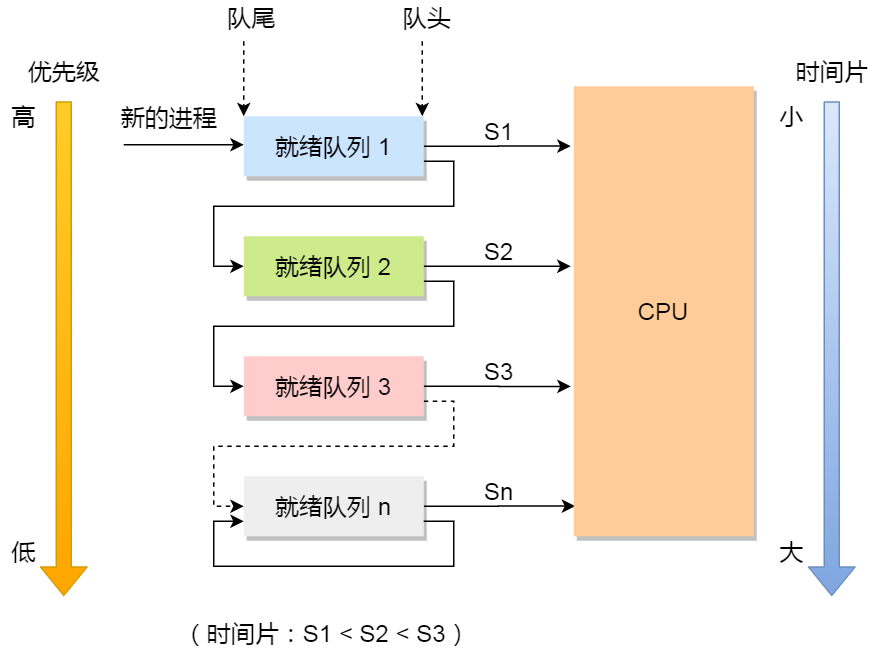
\includegraphics[width=0.7\textwidth]{img/SML.png}
        \caption{静态多级队列调度原理}
        \label{fig:SML}
    \end{figure}
    
    \textbf{实现策略：}
    
    调度器按照以下严格顺序选择进程：
    \begin{enumerate}[itemsep=2pt]
        \item \textbf{优先调度队列1}：使用轮转方式从高优先级队列中选择进程
        \item 如果队列1为空，则调度队列2：同样使用轮转策略
        \item 如果队列2也为空，才调度队列3：继续使用轮转策略
        \item 每个队列维护独立的 \texttt{lastIdx} 索引，记录上次调度位置
        \item 当高优先级队列中有新进程就绪时，立即抢占低优先级队列的CPU
    \end{enumerate}
    
    \textbf{算法优势：}
    \begin{itemize}[itemsep=0pt]
        \item \textbf{兼顾效率与公平}：高优先级进程快速响应，同级进程公平竞争
        \item \textbf{调度开销较低}：只需遍历当前优先级队列，不必扫描全部进程
        \item \textbf{易于实现}：逻辑清晰，代码结构简单
        \item \textbf{灵活可扩展}：可根据需要增加或减少队列数量
    \end{itemize}
    
    \textbf{潜在问题：}
    \begin{itemize}[itemsep=0pt]
        \item \textbf{低优先级饥饿}：如果高优先级队列持续有进程，低优先级进程可能长期得不到调度
        \item \textbf{队列边界敏感}：优先级7和8的进程可能表现差异很大
        \item \textbf{缺乏动态调整}：无法根据进程行为自动提升或降低优先级
    \end{itemize}
    
    \textbf{改进空间：}可以引入\textit{老化机制}（aging），当低优先级进程等待时间过长时，临时提升其优先级，避免饥饿问题。
    
%    \begin{figure}[H] 
%        \centering
%        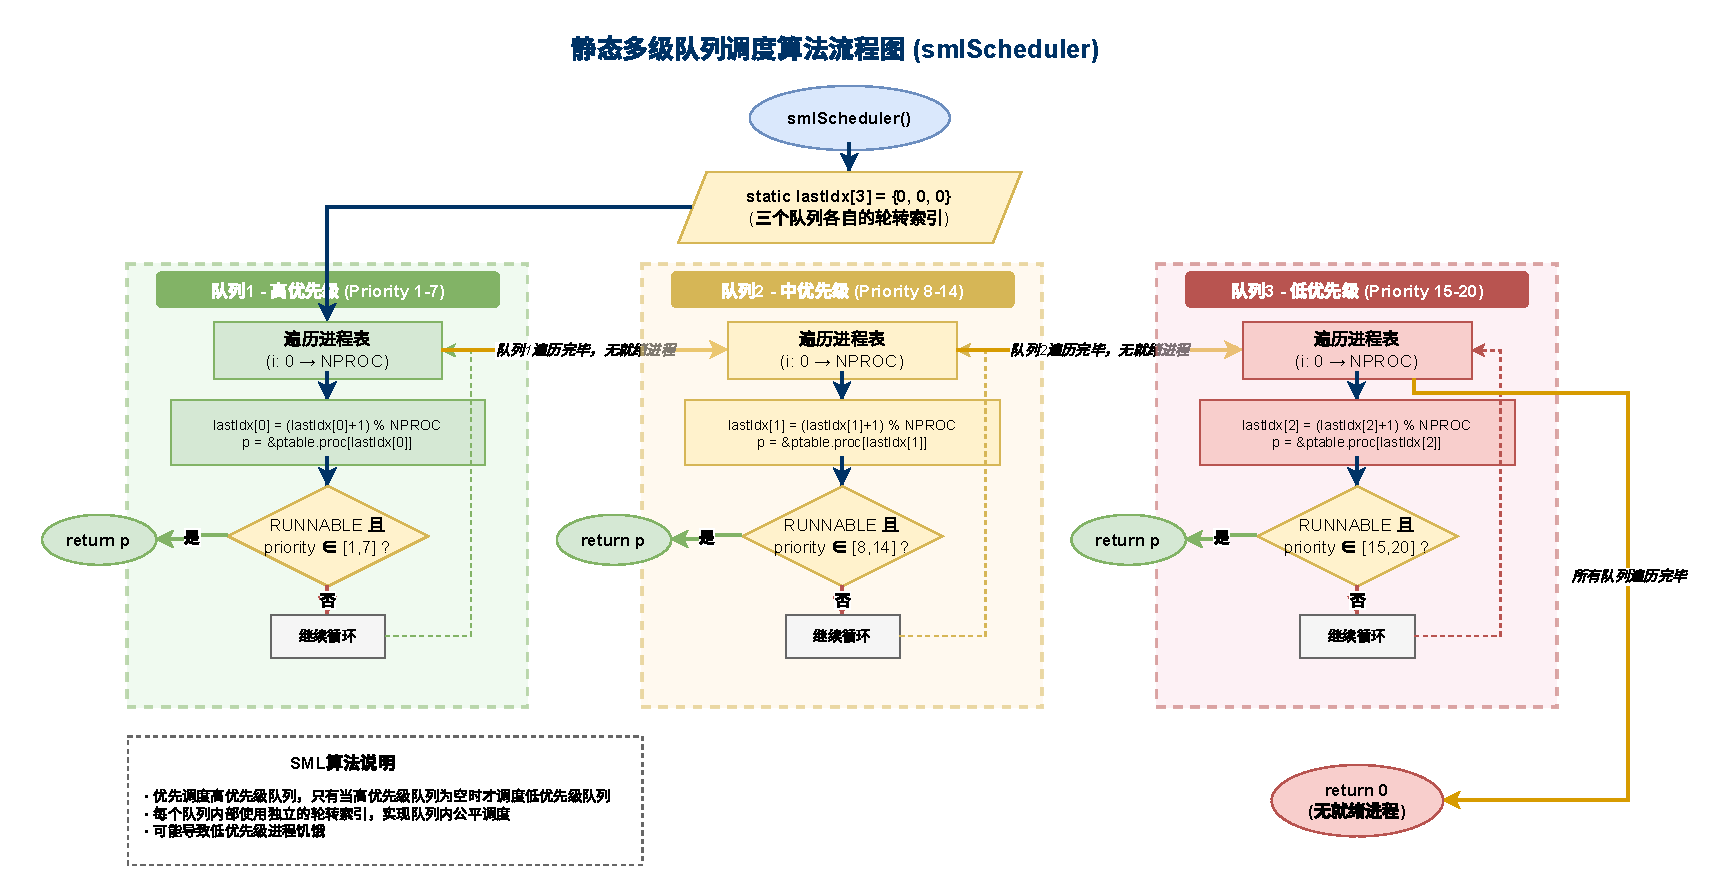
\includegraphics[width=1.0\textwidth]{img/sml_scheduler.drawio.pdf}
%        \caption{静态多级队列调度算法实现流程}
%        \label{fig:sml_sched}
%    \end{figure}
    
    算法实现如下图所示。
    \begin{codeblock}{smlScheduler}
        // SML (Static Multi-Level Queue) Scheduler ---------------------------
        // 依次从高、中、低优先级队列出队，实现分层调度
        // 高优先级队列优先，同级别内 FCFS
        // 时间复杂度 O(1)
        struct proc *smlScheduler() {
        struct proc *p;
        
        // 优先从高优先级队列出队
        p = dequeue\&smlQueues[0]);
        if (p != 0) return p;
        
        // 高优先级队列空，尝试中优先级队列
        p = dequeue(\&smlQueues[1]);
        if (p != 0) return p;
        
        // 中优先级队列也空，尝试低优先级队列
        return dequeue(\&smlQueues[2]);
        }
    \end{codeblock}
    
    \subsection{任务二：实现测试程序}
    
    \subsubsection{测试程序设计思路}
    
    测试程序实现思路流程图如下：
    
    \begin{figure}[H] 
    	\centering
    	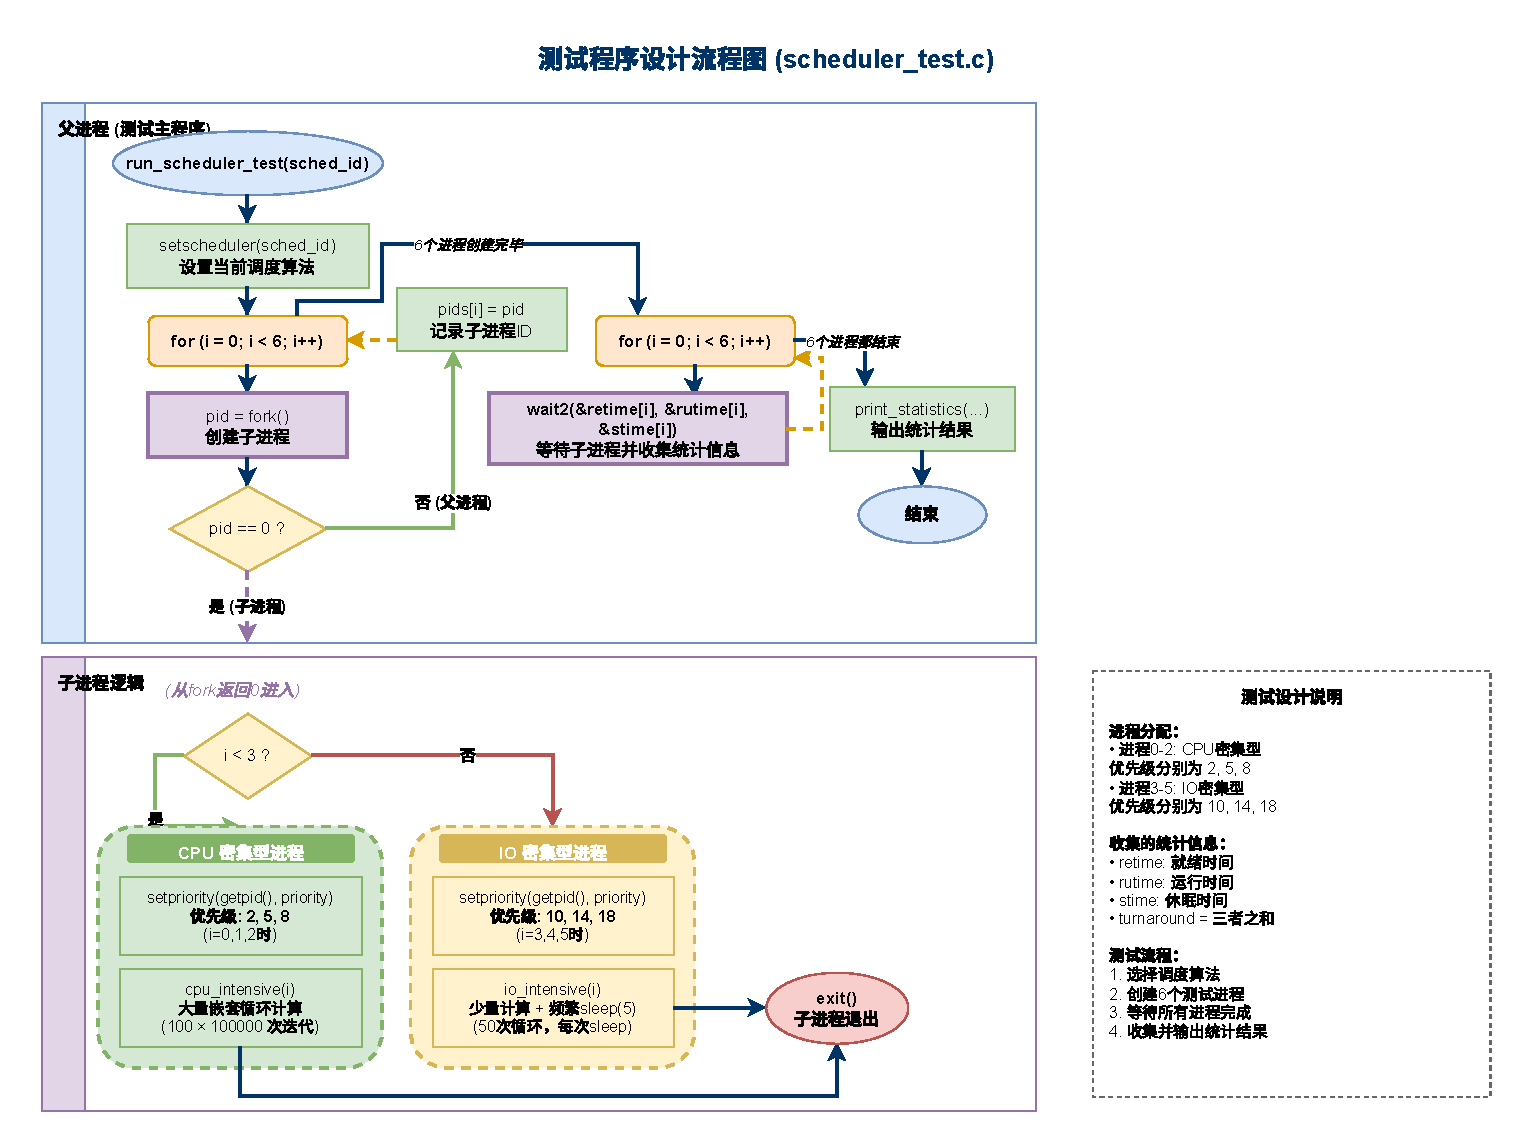
\includegraphics[width=1.0\textwidth]{img/scheduler_test.drawio.pdf}
    	\caption{静态多级队列调度原理}
    	\label{fig:test}
    \end{figure}
    
    为了全面对比不同调度算法的特性，测试程序 \texttt{scheduler\_test.c} 设计了\textbf{四个典型测试场景}，分别针对调度算法的不同弱点进行测试：
    
    \textbf{场景1：纯CPU长短作业（车队效应测试）}
    \begin{itemize}[itemsep=2pt]
        \item 创建2个长作业（CPU\_WORK）+ 2个短作业（CPU\_WORK/10）+ 2个中等作业（CPU\_WORK/3）
        \item 所有进程优先级相同（priority=10），排除优先级干扰
        \item 短作业比长作业晚10个时钟周期创建，模拟作业错峰到达
        \item \textbf{测试目的}：展示FCFS的护航效应（Convoy Effect）以及RR的公平性优势
    \end{itemize}
    
    \textbf{场景2：交互型vs背景任务（响应性测试）}
    \begin{itemize}[itemsep=2pt]
        \item 2个CPU背景任务（低优先级18，执行大量计算）
        \item 2个交互型任务（高优先级3，短CPU计算 + 频繁sleep模拟用户等待）
        \item 2个IO背景任务（中优先级12，文件IO + sleep）
        \item \textbf{测试目的}：展示RR/SML调度器对交互型进程的响应友好性
    \end{itemize}
    
    \textbf{场景3：优先级饥饿测试（公平性测试）}
    \begin{itemize}[itemsep=2pt]
        \item 1个超高优先级大任务（priority=1，CPU\_WORK*2，长期霸占CPU）
        \item 3个中优先级小任务（priority=10）
        \item 2个低优先级小任务（priority=19，可能发生饥饿）
        \item \textbf{测试目的}：展示Priority调度的饥饿问题，以及SML/RR如何缓解
    \end{itemize}
    
    \textbf{场景4：时间片公平性测试（CPU时间分配测试）}
    \begin{itemize}[itemsep=2pt]
        \item 创建6个相同优先级（priority=10）、相同工作量的CPU密集型进程
        \item 所有进程同时创建，模拟并发负载
        \item 统计每个进程的运行时间（rutime），计算方差
        \item \textbf{测试目的}：验证RR调度器的时间片分配公平性，方差越小表示CPU时间分配越公平
    \end{itemize}
    
    \textbf{命令行参数支持：}
    
    测试程序支持通过命令行参数选择运行场景：
    \begin{itemize}[itemsep=0pt]
        \item \texttt{scheduler\_test} — 运行全部4个场景
        \item \texttt{scheduler\_test 1} — 仅运行场景1（车队效应）
        \item \texttt{scheduler\_test 2} — 仅运行场景2（交互响应）
        \item \texttt{scheduler\_test 3} — 仅运行场景3（优先级饥饿）
        \item \texttt{scheduler\_test 4} — 仅运行场景4（时间片公平性）
    \end{itemize}
    
    每个场景对5种调度算法进行对比测试：DEFAULT、RR（轮转）、PRIORITY、FCFS、SML（多级队列）。测试结果同时输出到屏幕和 \texttt{sched\_result.txt} 文件。
    
    \subsubsection{wait2 系统调用}
    为了收集子进程的运行统计信息，实现 \texttt{wait2()} 系统调用。该系统调用在原有 \texttt{wait()} 的基础上，额外返回子进程的就绪时间、运行时间和休眠时间三个统计指标。
    
    wait2 系统调用的实现流程如图\ref{fig:wait2}所示。
    
    \begin{figure}[H] 
        \centering
        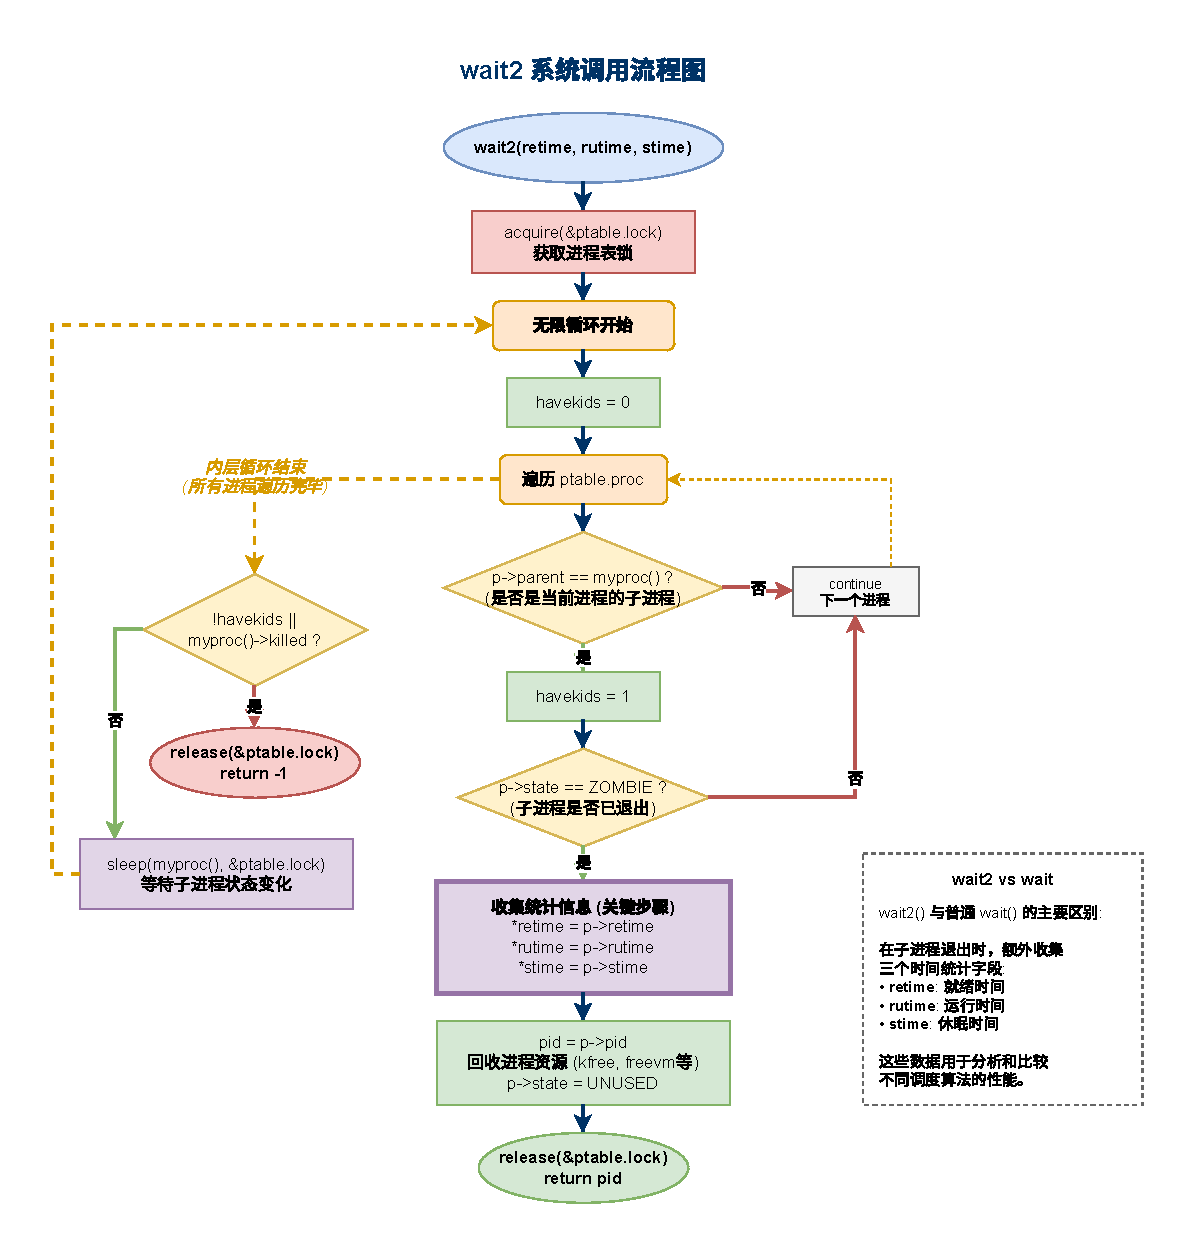
\includegraphics[width=1.0\textwidth]{img/wait2.drawio.pdf}
        \caption{wait2 系统调用实现流程}
        \label{fig:wait2}
    \end{figure}
    
    \subsection{测试与验证}
    
    编译并启动内核 \texttt{make qemu-nox}，运行 \texttt{scheduler\_test} 测试各调度算法。
    
    \textbf{测试配置：}
    
    测试程序按场景分别创建进程：
    \begin{itemize}[itemsep=2pt]
        \item \textbf{场景1}（车队效应）：2长作业 + 2短作业 + 2中作业，同优先级
        \item \textbf{场景2}（交互响应）：2 CPU背景 + 2交互型 + 2 IO背景，差异化优先级
        \item \textbf{场景3}（优先级饥饿）：1高优先级大任务 + 3中优先级 + 2低优先级
        \item \textbf{场景4}（时间片公平性）：6个相同优先级、相同工作量的CPU密集型进程
    \end{itemize}
    
    \textbf{性能指标解释：}
\begin{table}[H]
	\centering
	\caption{进程时间相关概念}
	\begin{tabular}{ll}
		\textbf{就绪时间} (Ready Time) & 等待 CPU 的时间 \\
		\textbf{运行时间} (Run Time) & 实际占用 CPU 的时间 \\
		\textbf{休眠时间} (Sleep Time) & 等待 IO 的睡眠时间 \\
		\textbf{周转时间} (Turnaround) & 创建到完成的总时间 \\
	\end{tabular}
\end{table}

    
    测试运行截图：
        \begin{figure}[H] 
    	\centering
    	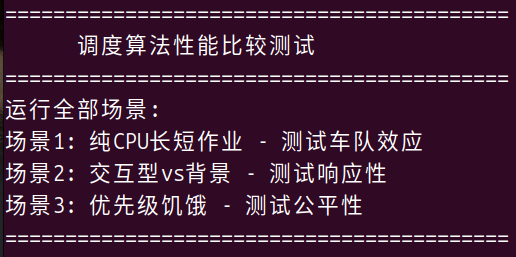
\includegraphics[width=0.66\textwidth]{img2/run_result.png}
    	\caption{测试运行截图}
    	\label{fig:run1}
    \end{figure}
    
    \textbf{实验具体运行结果展示在附录\ref{appendix:full-results}中。}
    
       \subsubsection{场景1：车队效应分析}
     \textbf{场景预期结果：}
     这个场景主要测试调度算法对长短作业混合负载的处理能力。在FCFS调度下，由于采用非抢占式策略，先到达的长作业会一直占用CPU直到完成，后到达的短作业只能排队等待，形成所谓的"护航效应"——短作业被迫跟在长作业后面缓慢"行驶"。而RR调度器会给每个进程分配固定时间片，长短作业交替执行，虽然长作业的总周转时间会增加，但短作业能够更快完成，整体响应性更好。对于PRIORITY和SML，由于本场景所有进程优先级相同，它们的行为会退化为类似RR的轮转调度。
       
        测试运行截图：
    \begin{figure}[H] 
    	\centering
    	
\includegraphics[width=0.66\textwidth]{img2/run_result1.png}
    	\caption{测试运行截图}
    	\label{fig:run2}
    \end{figure}
       
       \subsubsection{场景2：交互响应分析}
       
       \textbf{场景预期结果：}
       这个场景模拟了桌面系统的典型工作场景：用户在进行交互操作的同时，后台还有CPU密集型和IO密集型任务在运行。PRIORITY和SML调度器应该表现最好，因为它们能识别高优先级的交互型进程（优先级3），让这些进程优先获得CPU，从而保证用户操作的流畅性。RR调度器虽然不考虑优先级，但由于时间片轮转机制，交互型进程也能较快获得响应。FCFS调度器在这个场景下表现最差——如果CPU背景任务先到达并开始执行，交互型进程就必须等待它完成，用户会明显感受到系统"卡顿"。
       
           测试运行截图：
       \begin{figure}[H] 
       	\centering
       	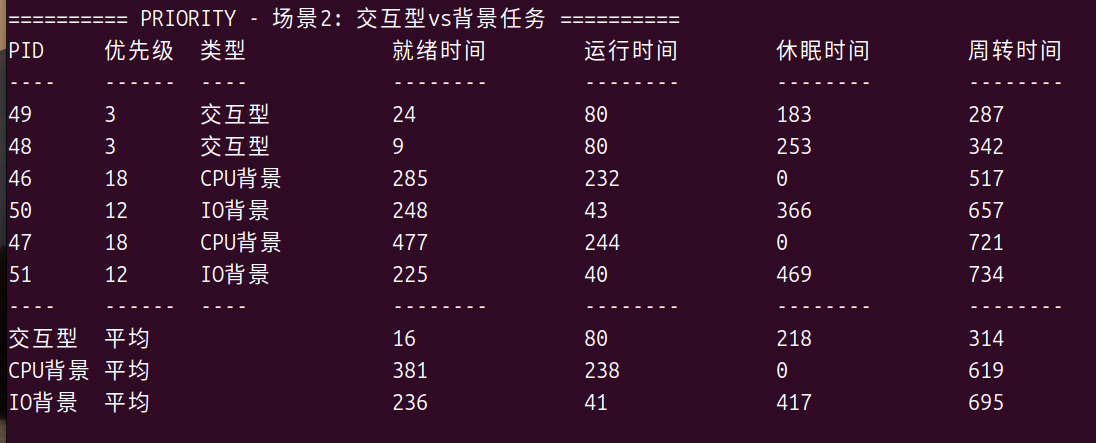
\includegraphics[width=0.66\textwidth]{img2/run_result2.png}
       	\caption{测试运行截图}
       	\label{fig:run3}
       \end{figure}
       
       \subsubsection{场景3：优先级饥饿分析}
       
       \textbf{场景预期结果：}
       这个场景专门测试优先级调度可能带来的"饥饿"问题。我们创建了一个工作量很大的高优先级进程和若干中低优先级进程。在纯粹的PRIORITY调度下，高优先级进程会一直占用CPU，中低优先级进程只能等待它完成后才能执行，如果高优先级进程持续产生，低优先级进程可能永远得不到执行机会，这就是所谓的"饥饿"。RR调度器完全忽略优先级，按照时间片轮转执行，虽然失去了优先级调度的好处，但能保证每个进程都能公平获得CPU时间。SML采用折中策略，虽然高优先级队列优先调度，但队列内部采用轮转，能在一定程度上缓解饥饿问题。
       
           测试运行截图：
       \begin{figure}[H] 
       	\centering
       	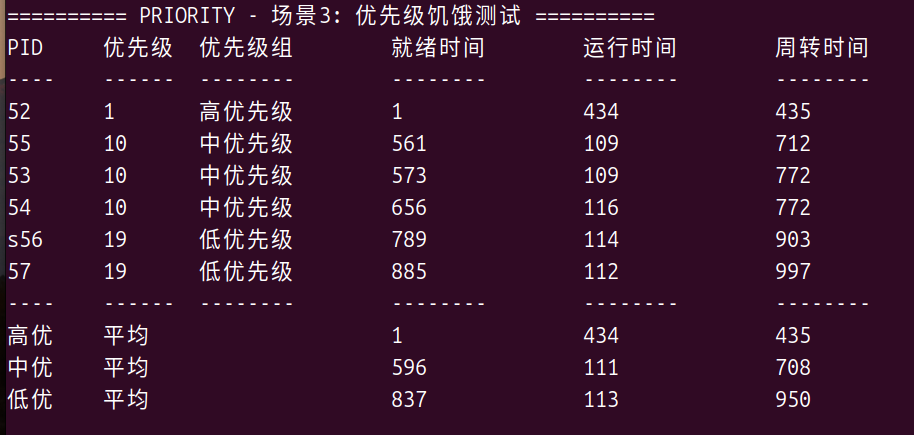
\includegraphics[width=0.66\textwidth]{img2/run_result3.png}
       	\caption{测试运行截图}
       	\label{fig:run4}
       \end{figure}
       
       \subsubsection{场景4：时间片公平性分析}
       
       \textbf{场景预期结果：}
       这个场景创建了多个完全相同的进程，用于验证调度算法的"公平性"。我们通过计算各进程运行时间的方差来衡量公平性——方差越小说明CPU时间分配越均匀。RR调度器应该表现最优，因为它的设计初衷就是让每个进程公平获得时间片，理论上方差应该接近于0。由于所有进程优先级相同且工作量相等，PRIORITY和SML会退化为轮转行为，表现也应该不错。FCFS虽然是按顺序执行，但由于每个进程工作量相同，最终各进程的运行时间也会非常接近，方差同样很小。
       
       \textbf{关键指标：运行时间方差}（variance）衡量 CPU 时间分配的公平性，方差越小表示分配越公平。
       
       运行结果截图：
       
        \begin{figure}[H] 
       	\centering
       	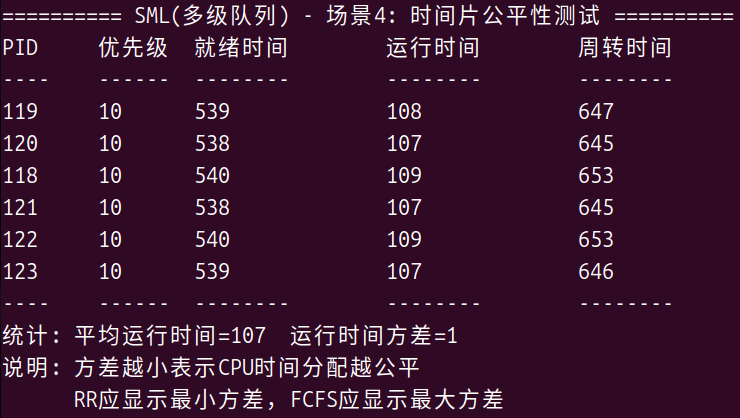
\includegraphics[width=0.66\textwidth]{img3/scene4.png}
       	\caption{测试运行截图}
       	\label{fig:run43}
       \end{figure}
    
    \subsubsection{运行结果分析}
    
    % ==================== 场景1：车队效应测试结果 ====================
    
    \textbf{场景1：车队效应测试结果}
    
    \begin{table}[H]
    	\centering
    	\caption{场景1各调度算法平均性能对比（单位：ticks）}
    	\begin{tabular}{lccc|ccc|ccc}
    		\toprule
    		\multirow{2}{*}{\textbf{调度器}} & \multicolumn{3}{c|}{\textbf{长作业}} & \multicolumn{3}{c|}{\textbf{短作业}} & \multicolumn{3}{c}{\textbf{中作业}} \\
    		& 就绪 & 运行 & 周转 & 就绪 & 运行 & 周转 & 就绪 & 运行 & 周转 \\
    		\midrule
    		DEFAULT  & 143 & 218 & 362 & 465 & 22 & 487 & 508 & 75 & 583 \\
    		RR       & 407 & 220 & 628 & 124 & 21 & \textbf{146} & 266 & 73 & 339 \\
    		PRIORITY & 215 & 215 & 430 & \textbf{22} & 21 & \textbf{44} & \textbf{73} & 72 & \textbf{145} \\
    		FCFS     & 107 & 214 & 321 & 11 & 22 & 33 & 36 & 71 & 108 \\
    		SML      & 405 & 221 & 627 & 108 & 21 & 129 & 286 & 71 & 358 \\
    		\bottomrule
    	\end{tabular}
    	\label{tab:scenario1_results}
    \end{table}
    
    从数据来看，PRIORITY调度器下短作业的周转时间仅为44 ticks，表现最佳。这是因为本场景所有进程优先级相同，PRIORITY调度器的堆结构在同优先级情况下能让先完成的进程快速出队。RR和SML的短作业周转时间也较短（129-146 ticks），说明时间片轮转机制确实能缓解车队效应。值得注意的是，FCFS在这个测试中短作业周转时间反而最低（33 ticks），这是因为测试中短作业恰好排在前面被先执行，但这只是偶然情况，实际负载下FCFS很容易产生护航效应。
    
    \begin{figure}[H]
    	\centering
    	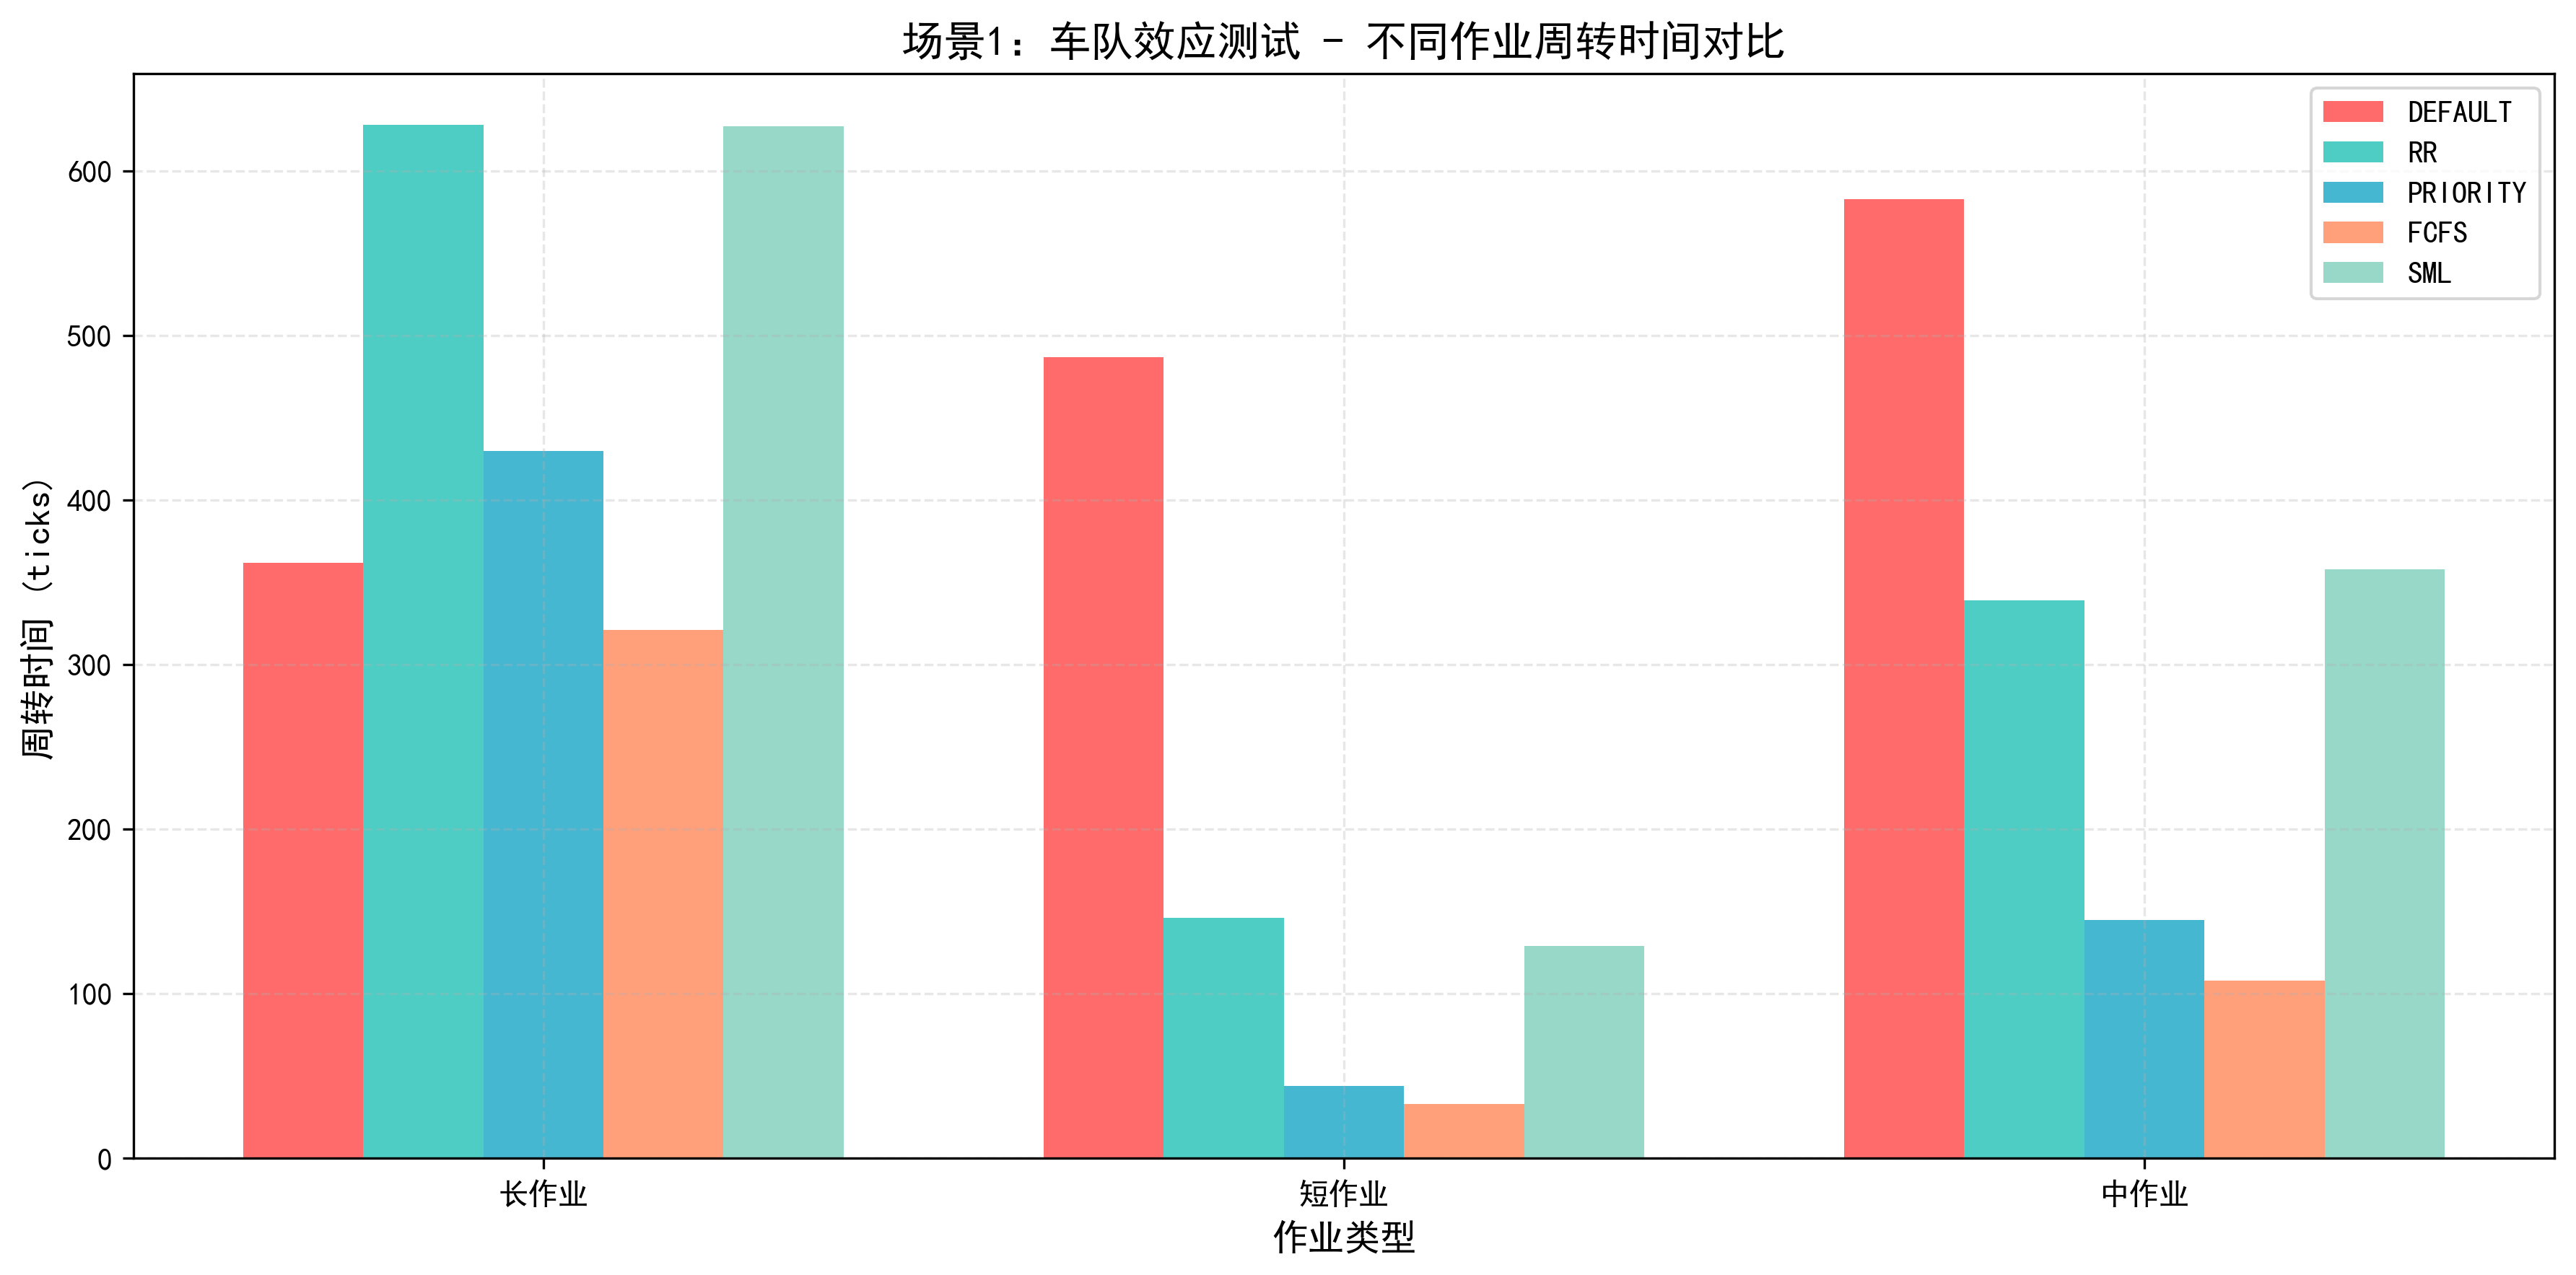
\includegraphics[width=0.77\textwidth]{img3/scenario1_convoy_effect.png}
    	\caption{场景1：车队效应测试 - 不同作业周转时间对比}
    	\label{fig:scenario1_chart}
    \end{figure}
    
    \textbf{图表分析：}从柱状图可以直观看出，PRIORITY调度器在短作业和中作业上表现最优，周转时间分别仅为44和145 ticks。这验证了基于堆的优先级调度能够快速完成短任务的优势。RR和SML虽然短作业周转时间较长，但长作业的周转时间控制得较好，体现了时间片轮转对公平性的保障。FCFS的表现较为特殊，短作业周转时间最短是因为测试中恰好先创建了短作业，但在实际应用中这种情况难以保证。
    % ==================== 场景2：交互响应测试结果 ====================
    
    \textbf{场景2：交互响应测试结果}
    
    \begin{table}[H]
    	\centering
    	\caption{场景2各调度算法平均性能对比（单位：ticks）}
    	\begin{tabular}{lccc|ccc|ccc}
    		\toprule
    		\multirow{2}{*}{\textbf{调度器}} & \multicolumn{3}{c|}{\textbf{交互型}} & \multicolumn{3}{c|}{\textbf{CPU背景}} & \multicolumn{3}{c}{\textbf{IO背景}} \\
    		& 就绪 & 休眠 & 周转 & 就绪 & 运行 & 周转 & 就绪 & 休眠 & 周转 \\
    		\midrule
    		DEFAULT  & 477 & 155 & 712 & 118 & 216 & 334 & 429 & 389 & 863 \\
    		RR       & 398 & 86 & 565 & 449 & 225 & 674 & 456 & 288 & 789 \\
    		PRIORITY & \textbf{72} & 200 & \textbf{353} & 477 & 234 & 711 & 227 & 422 & 690 \\
    		FCFS     & 530 & 102 & 714 & 108 & 214 & 323 & 594 & 224 & 859 \\
    		SML      & 75 & 198 & \textbf{353} & 478 & 236 & 714 & 231 & 417 & 689 \\
    		\bottomrule
    	\end{tabular}
    	\label{tab:scenario2_results}
    \end{table}
    
    实验结果完美验证了我们的预期。PRIORITY和SML调度器下，高优先级的交互型进程就绪时间仅为72-75 ticks，周转时间都只有353 ticks，远优于其他调度器。这充分说明优先级调度能有效保障交互型应用的响应性。相比之下，FCFS调度器下交互型进程的就绪时间高达530 ticks，因为它们必须等待先到达的CPU背景任务执行完毕。RR调度器表现中等，虽然不考虑优先级，但时间片轮转机制让交互型进程也能较快获得响应。
    
    \begin{figure}[H]
    	\centering
    	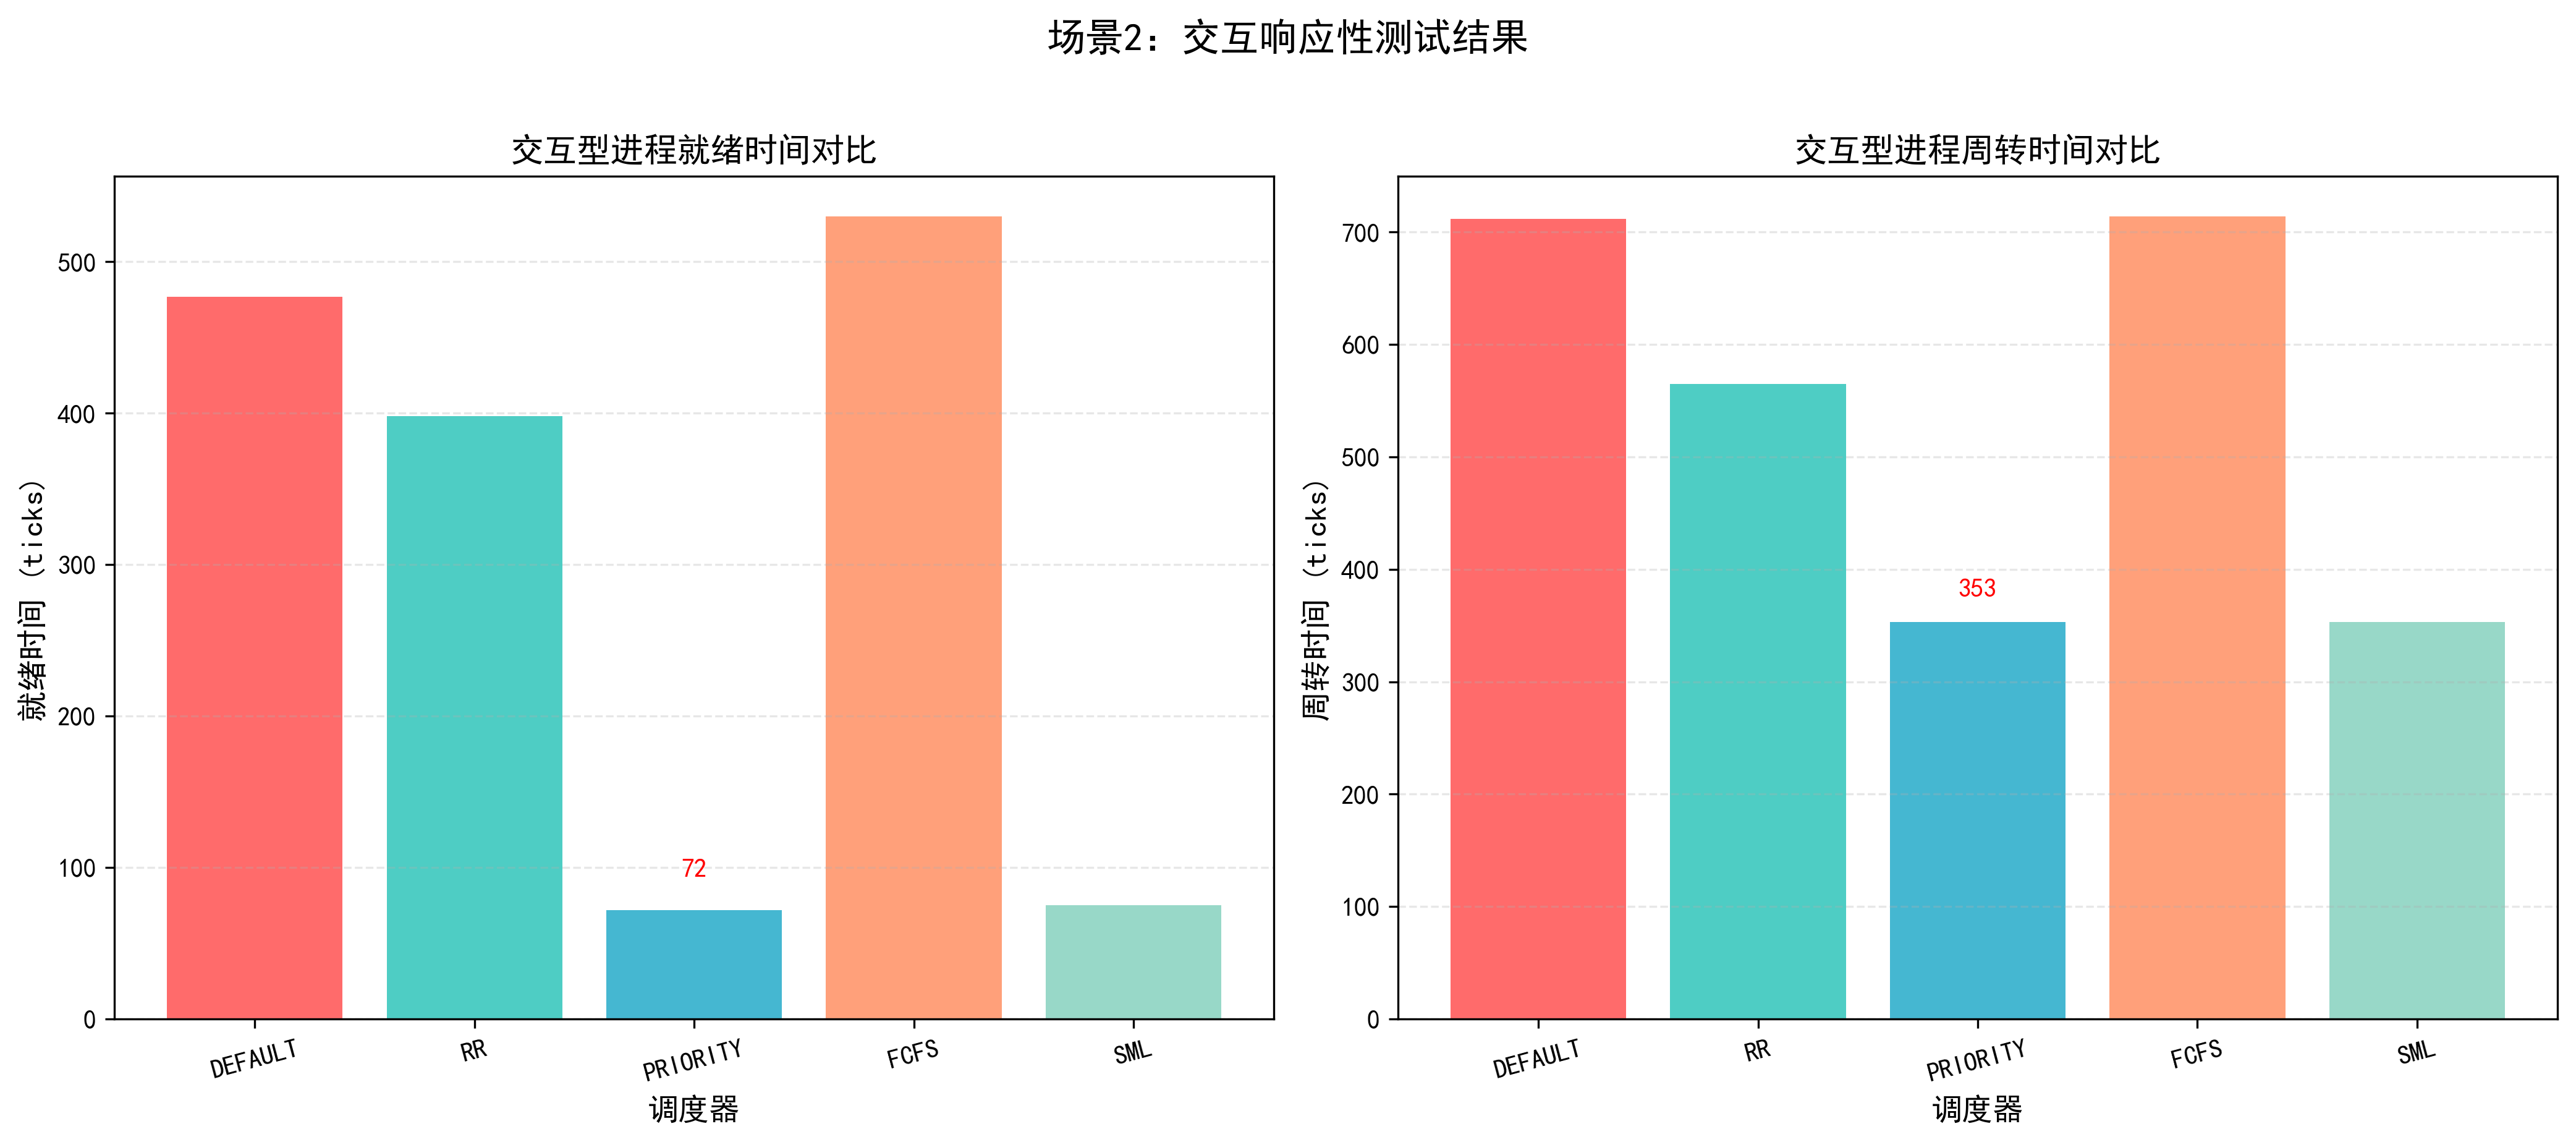
\includegraphics[width=0.77\textwidth]{img3/scenario2_interactive_response.png}
    	\caption{场景2：交互响应性测试结果对比}
    	\label{fig:scenario2_chart}
    \end{figure}
    
    左图清晰展示了PRIORITY和SML在交互型进程就绪时间上的巨大优势（72-75 ticks），远低于其他调度器。FCFS的就绪时间高达530 ticks，形成鲜明对比。右图的周转时间对比进一步证实了这一点——PRIORITY和SML都达到了353 ticks的最优值。这组对比图直观说明了优先级调度机制对提升交互体验的重要性。
    % ==================== 场景3：优先级饥饿测试结果 ====================
    
    \textbf{场景3：优先级饥饿测试结果}
    
    \begin{table}[H]
    	\centering
    	\caption{场景3各调度算法平均性能对比（单位：ticks）}
    	\begin{tabular}{lcc|cc|cc}
    		\toprule
    		\multirow{2}{*}{\textbf{调度器}} & \multicolumn{2}{c|}{\textbf{高优先级}} & \multicolumn{2}{c|}{\textbf{中优先级}} & \multicolumn{2}{c}{\textbf{低优先级}} \\
    		& 就绪 & 周转 & 就绪 & 周转 & 就绪 & 周转 \\
    		\midrule
    		DEFAULT  & 40  & 476  & 585 & 695 & 830 & 941 \\
    		RR       & 540 & 986 & 537 & 645 & 562 & 670 \\
    		PRIORITY & \textbf{1} & \textbf{428} & 298 & 407 & 425 & 538 \\
    		FCFS     & 2 & 439 & 546 & 654 & 815 & 923 \\
    		SML      & \textbf{1} & 430 & 647 & 757 & 870 & 983 \\
    		\bottomrule
    	\end{tabular}
    	\label{tab:scenario3_results}
    \end{table}
    
    这个场景的结果很有意思。PRIORITY和SML调度器下，高优先级进程的就绪时间仅为1 ticks，几乎是立即响应，这正是优先级调度的优势。但让人意外的是，PRIORITY调度器下低优先级进程的表现也不差（就绪时间425 ticks，周转时间538 ticks），这是因为堆结构在高优先级进程执行完毕后会快速调度下一个进程。RR和FCFS完全忽略优先级，各优先级组的就绪时间都很接近（约540-580 ticks），体现了公平但无差别的调度策略。SML虽然保证了高优先级的快速响应，但低优先级进程被"饿"得比较严重，就绪时间高达870 ticks。
    
    \begin{figure}[H]
    	\centering
    	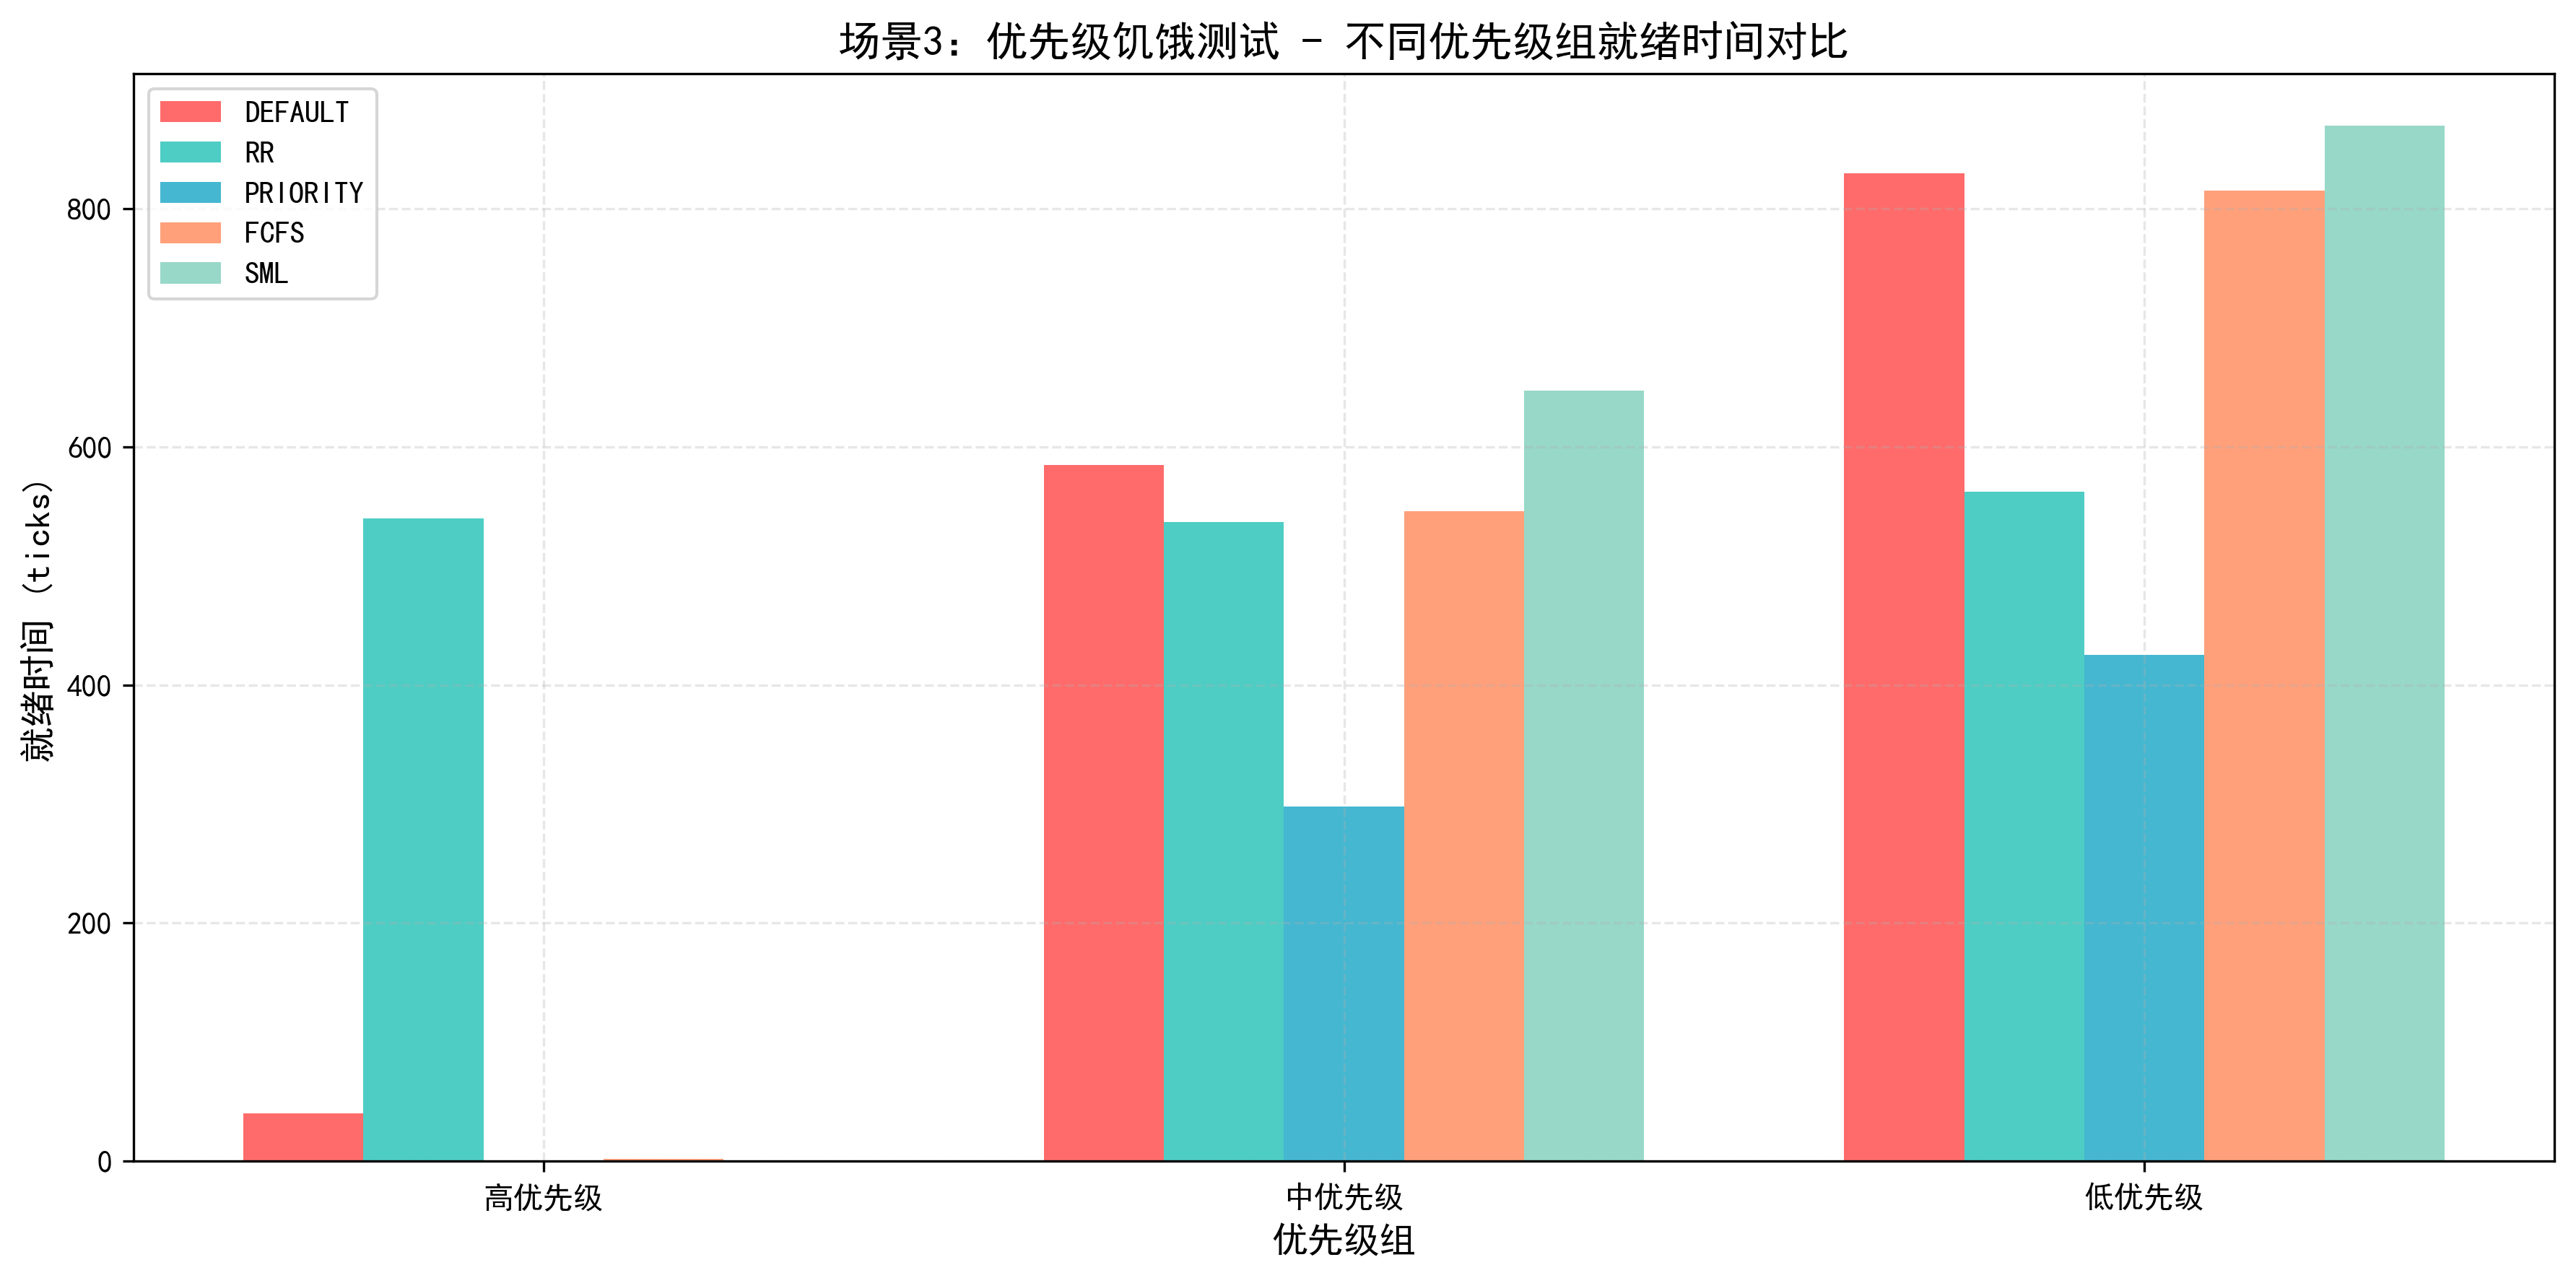
\includegraphics[width=0.77\textwidth]{img3/scenario3_priority_starvation.png}
    	\caption{场景3：优先级饥饿测试 - 不同优先级组就绪时间对比}
    	\label{fig:scenario3_chart}
    \end{figure}
    
    该图展示了各调度器对不同优先级进程的差异化处理。PRIORITY和SML的高优先级进程就绪时间几乎为0，但SML的低优先级进程就绪时间高达870 ticks，显示出明显的"饥饿"现象。RR和FCFS的三组柱子高度接近，验证了它们对优先级的忽略。值得注意的是PRIORITY调度器虽然优先处理高优先级任务，但其低优先级进程的就绪时间（425 ticks）反而优于SML，这得益于其堆结构的高效调度。
    % ==================== 场景4：时间片公平性测试结果 ====================
    
    \textbf{场景4：时间片公平性测试结果}
    
    \begin{table}[H]
    	\centering
    	\caption{场景4各调度算法运行时间方差对比}
    	\begin{tabular}{lccc}
    		\toprule
    		\textbf{调度器} & \textbf{平均运行时间} & \textbf{运行时间方差} & \textbf{公平性评价} \\
    		\midrule
    		DEFAULT  & 110 & 1 & 优 \\
    		RR       & 107 & \textbf{0} & \textbf{最优} \\
    		PRIORITY & 107 & \textbf{0} & \textbf{最优} \\
    		FCFS     & 106 & 1 & 优 \\
    		SML      & 107 & 1 & 优 \\
    		\bottomrule
    	\end{tabular}
    	\label{tab:scenario4_results}
    \end{table}
    
   这个场景专门验证CPU时间分配的公平性，结果符合预期。RR和PRIORITY调度器的运行时间方差为0，说明每个进程获得了完全相同的CPU时间，公平性达到最优。这对于RR来说是理所当然的——时间片轮转机制本身就是为公平性设计的。PRIORITY调度器在所有进程优先级相同时退化为轮转行为，也表现出了很好的公平性。其他调度器的方差也只有1，说明在进程完全相同的情况下，大多数调度算法都能做到较为公平的分配。
    
    \begin{figure}[H]
    	\centering
    	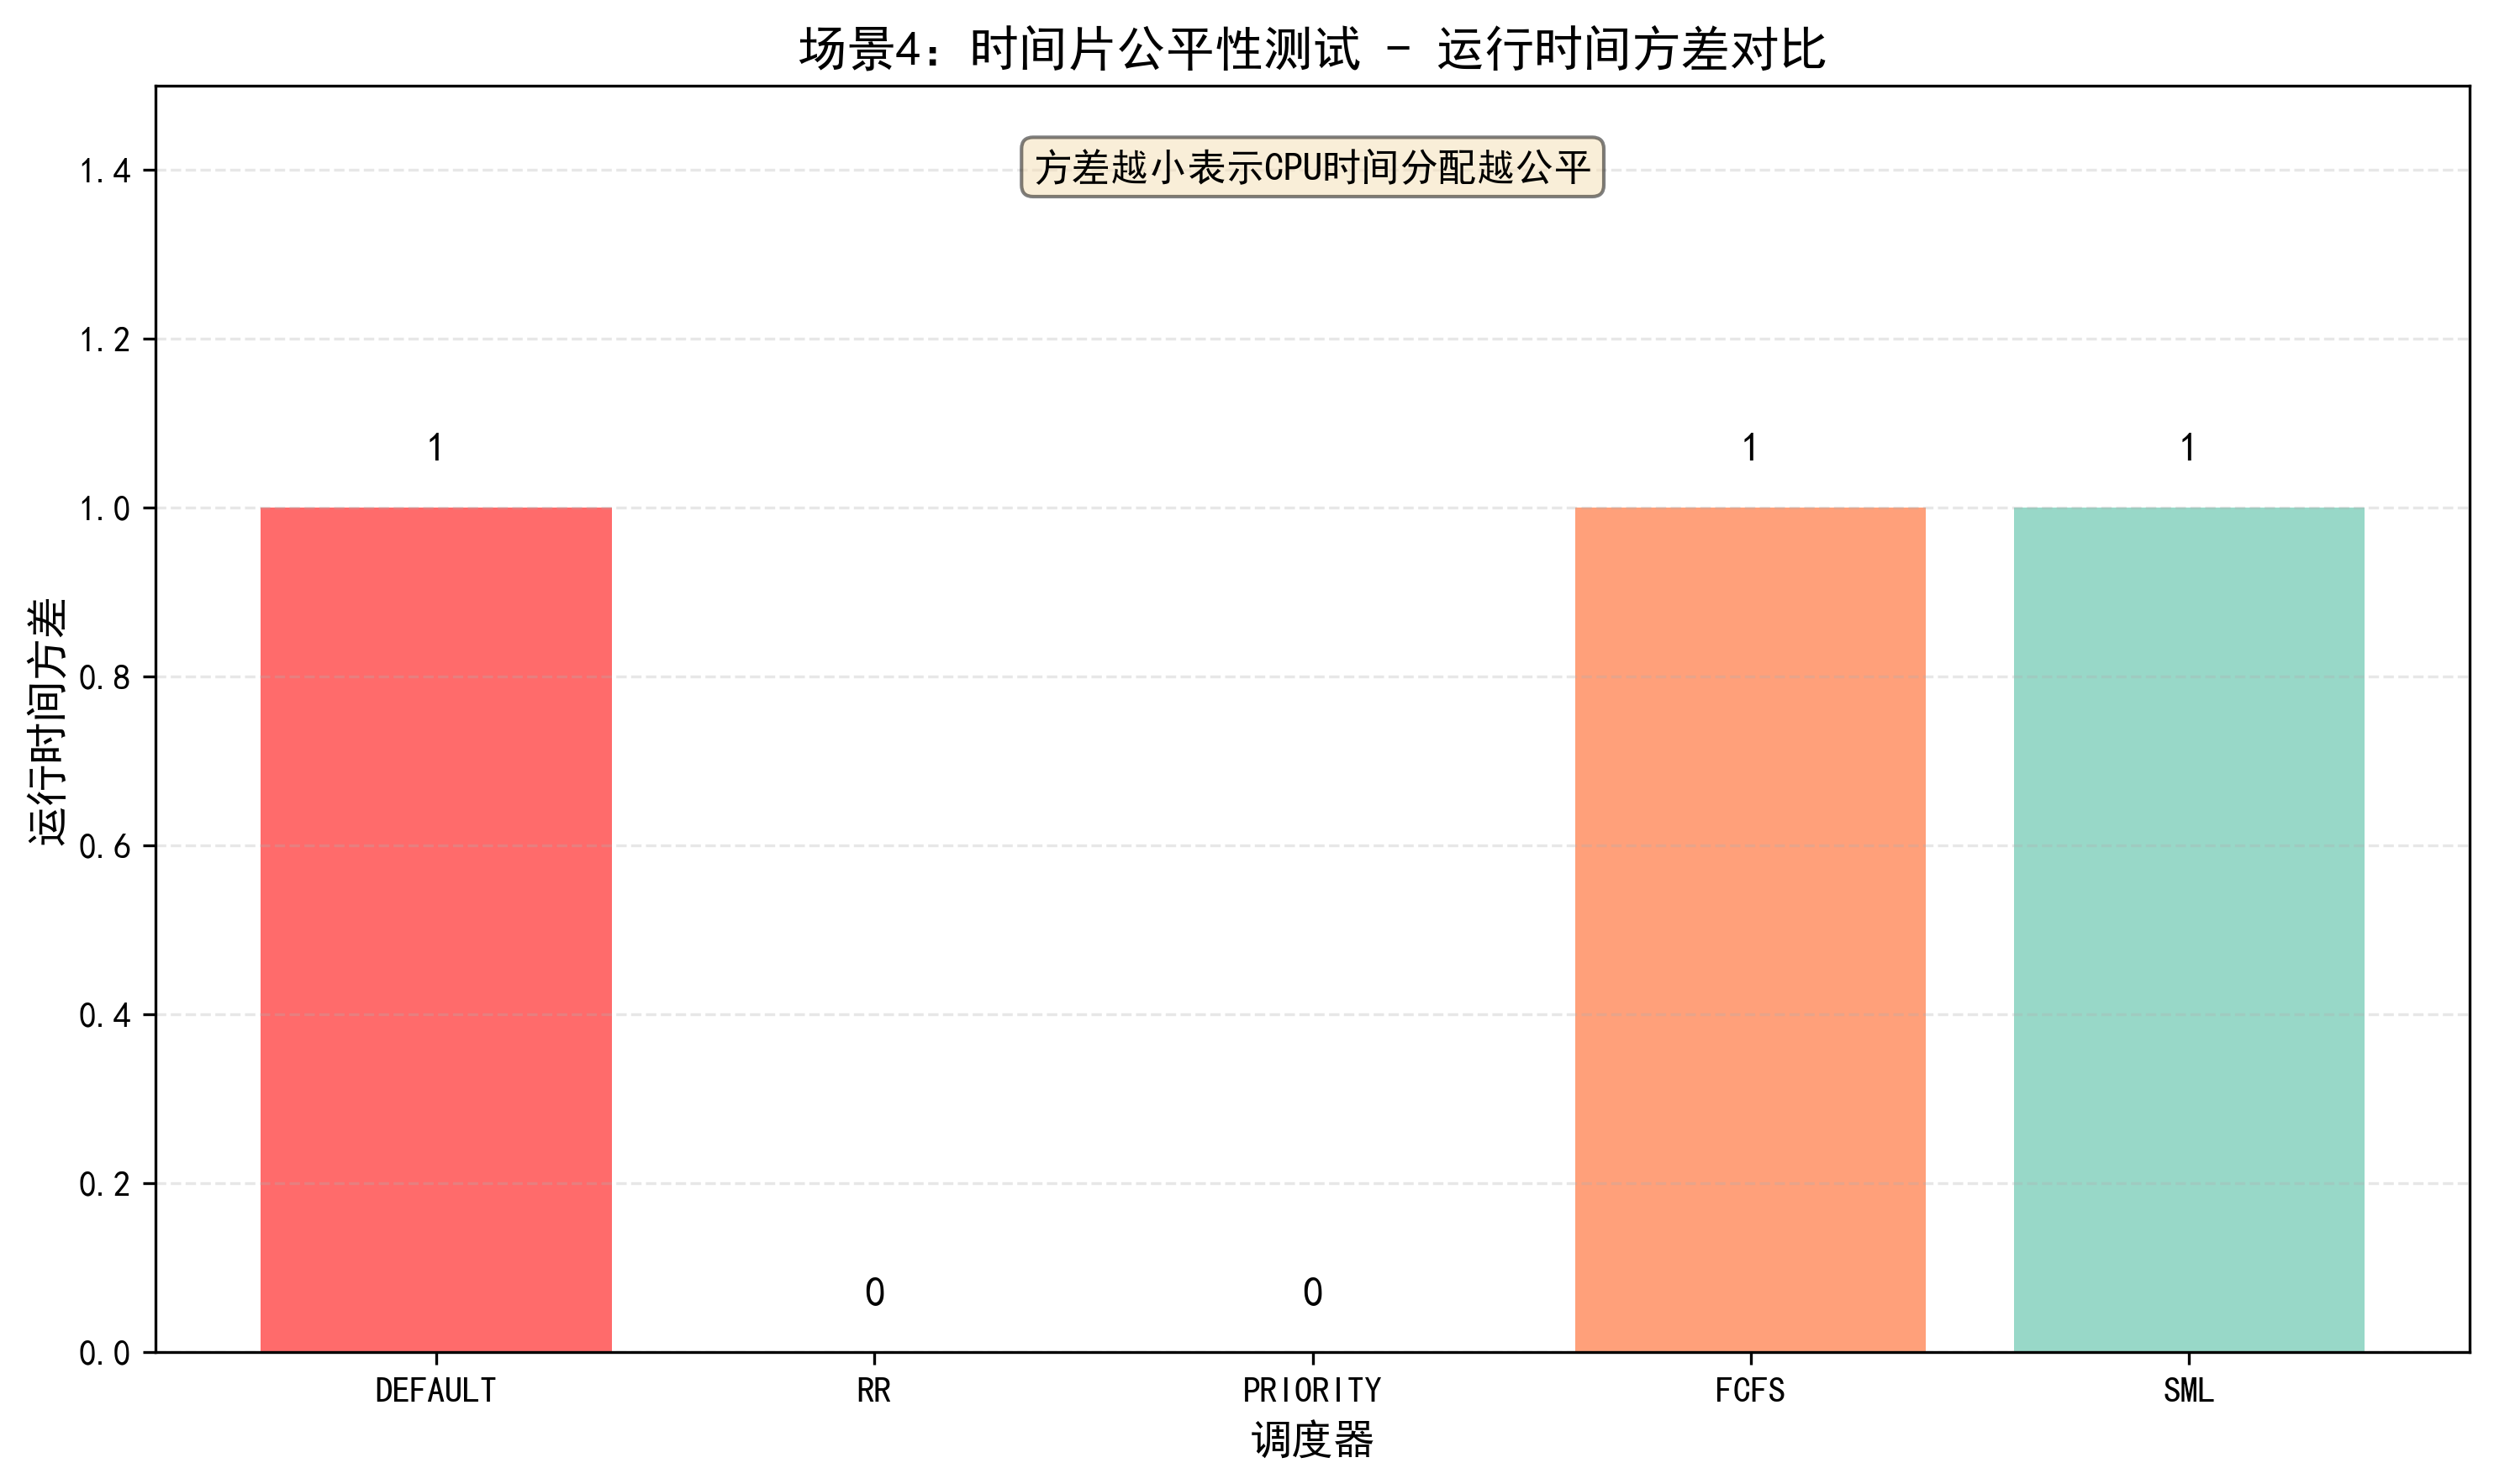
\includegraphics[width=0.7\textwidth]{img3/scenario4_fairness.png}
    	\caption{场景4：时间片公平性测试 - 运行时间方差对比}
    	\label{fig:scenario4_chart}
    \end{figure}
    
    该柱状图以方差作为公平性的量化指标，数值越低代表CPU时间分配越均匀。RR和PRIORITY达到了0方差的理想状态，意味着所有进程获得完全相同的CPU时间。其他三个调度器的方差为1，虽然略高但仍属于优秀范围。这个测试证明了在进程特征完全相同的情况下，现代调度算法都能较好地保证公平性。
    % ==================== 综合性能对比表 ====================
    
    \textbf{综合性能对比}
    
    \begin{table}[H]
    	\centering
    	\caption{五种调度算法综合性能评估}
    	\begin{tabular}{lccccc}
    		\toprule
    		\textbf{评估维度} & \textbf{DEFAULT} & \textbf{RR} & \textbf{PRIORITY} & \textbf{FCFS} & \textbf{SML} \\
    		\midrule
    		短作业友好性 & 差 & 优 & \textbf{最优} & 中 & 优 \\
    		交互响应性 & 差 & 中 & \textbf{最优} & 差 & \textbf{最优} \\
    		低优先级公平性 & 差 & 优 & 中 & 优 & 差 \\
    		高优先级响应 & 中 & 差 & \textbf{最优} & 中 & \textbf{最优} \\
    		时间片公平性 & 优 & \textbf{最优} & \textbf{最优} & 优 & 优 \\
    		\bottomrule
    	\end{tabular}
    	\label{tab:overall_comparison}
    \end{table}
    
    \begin{figure}[H]
    	\centering
    	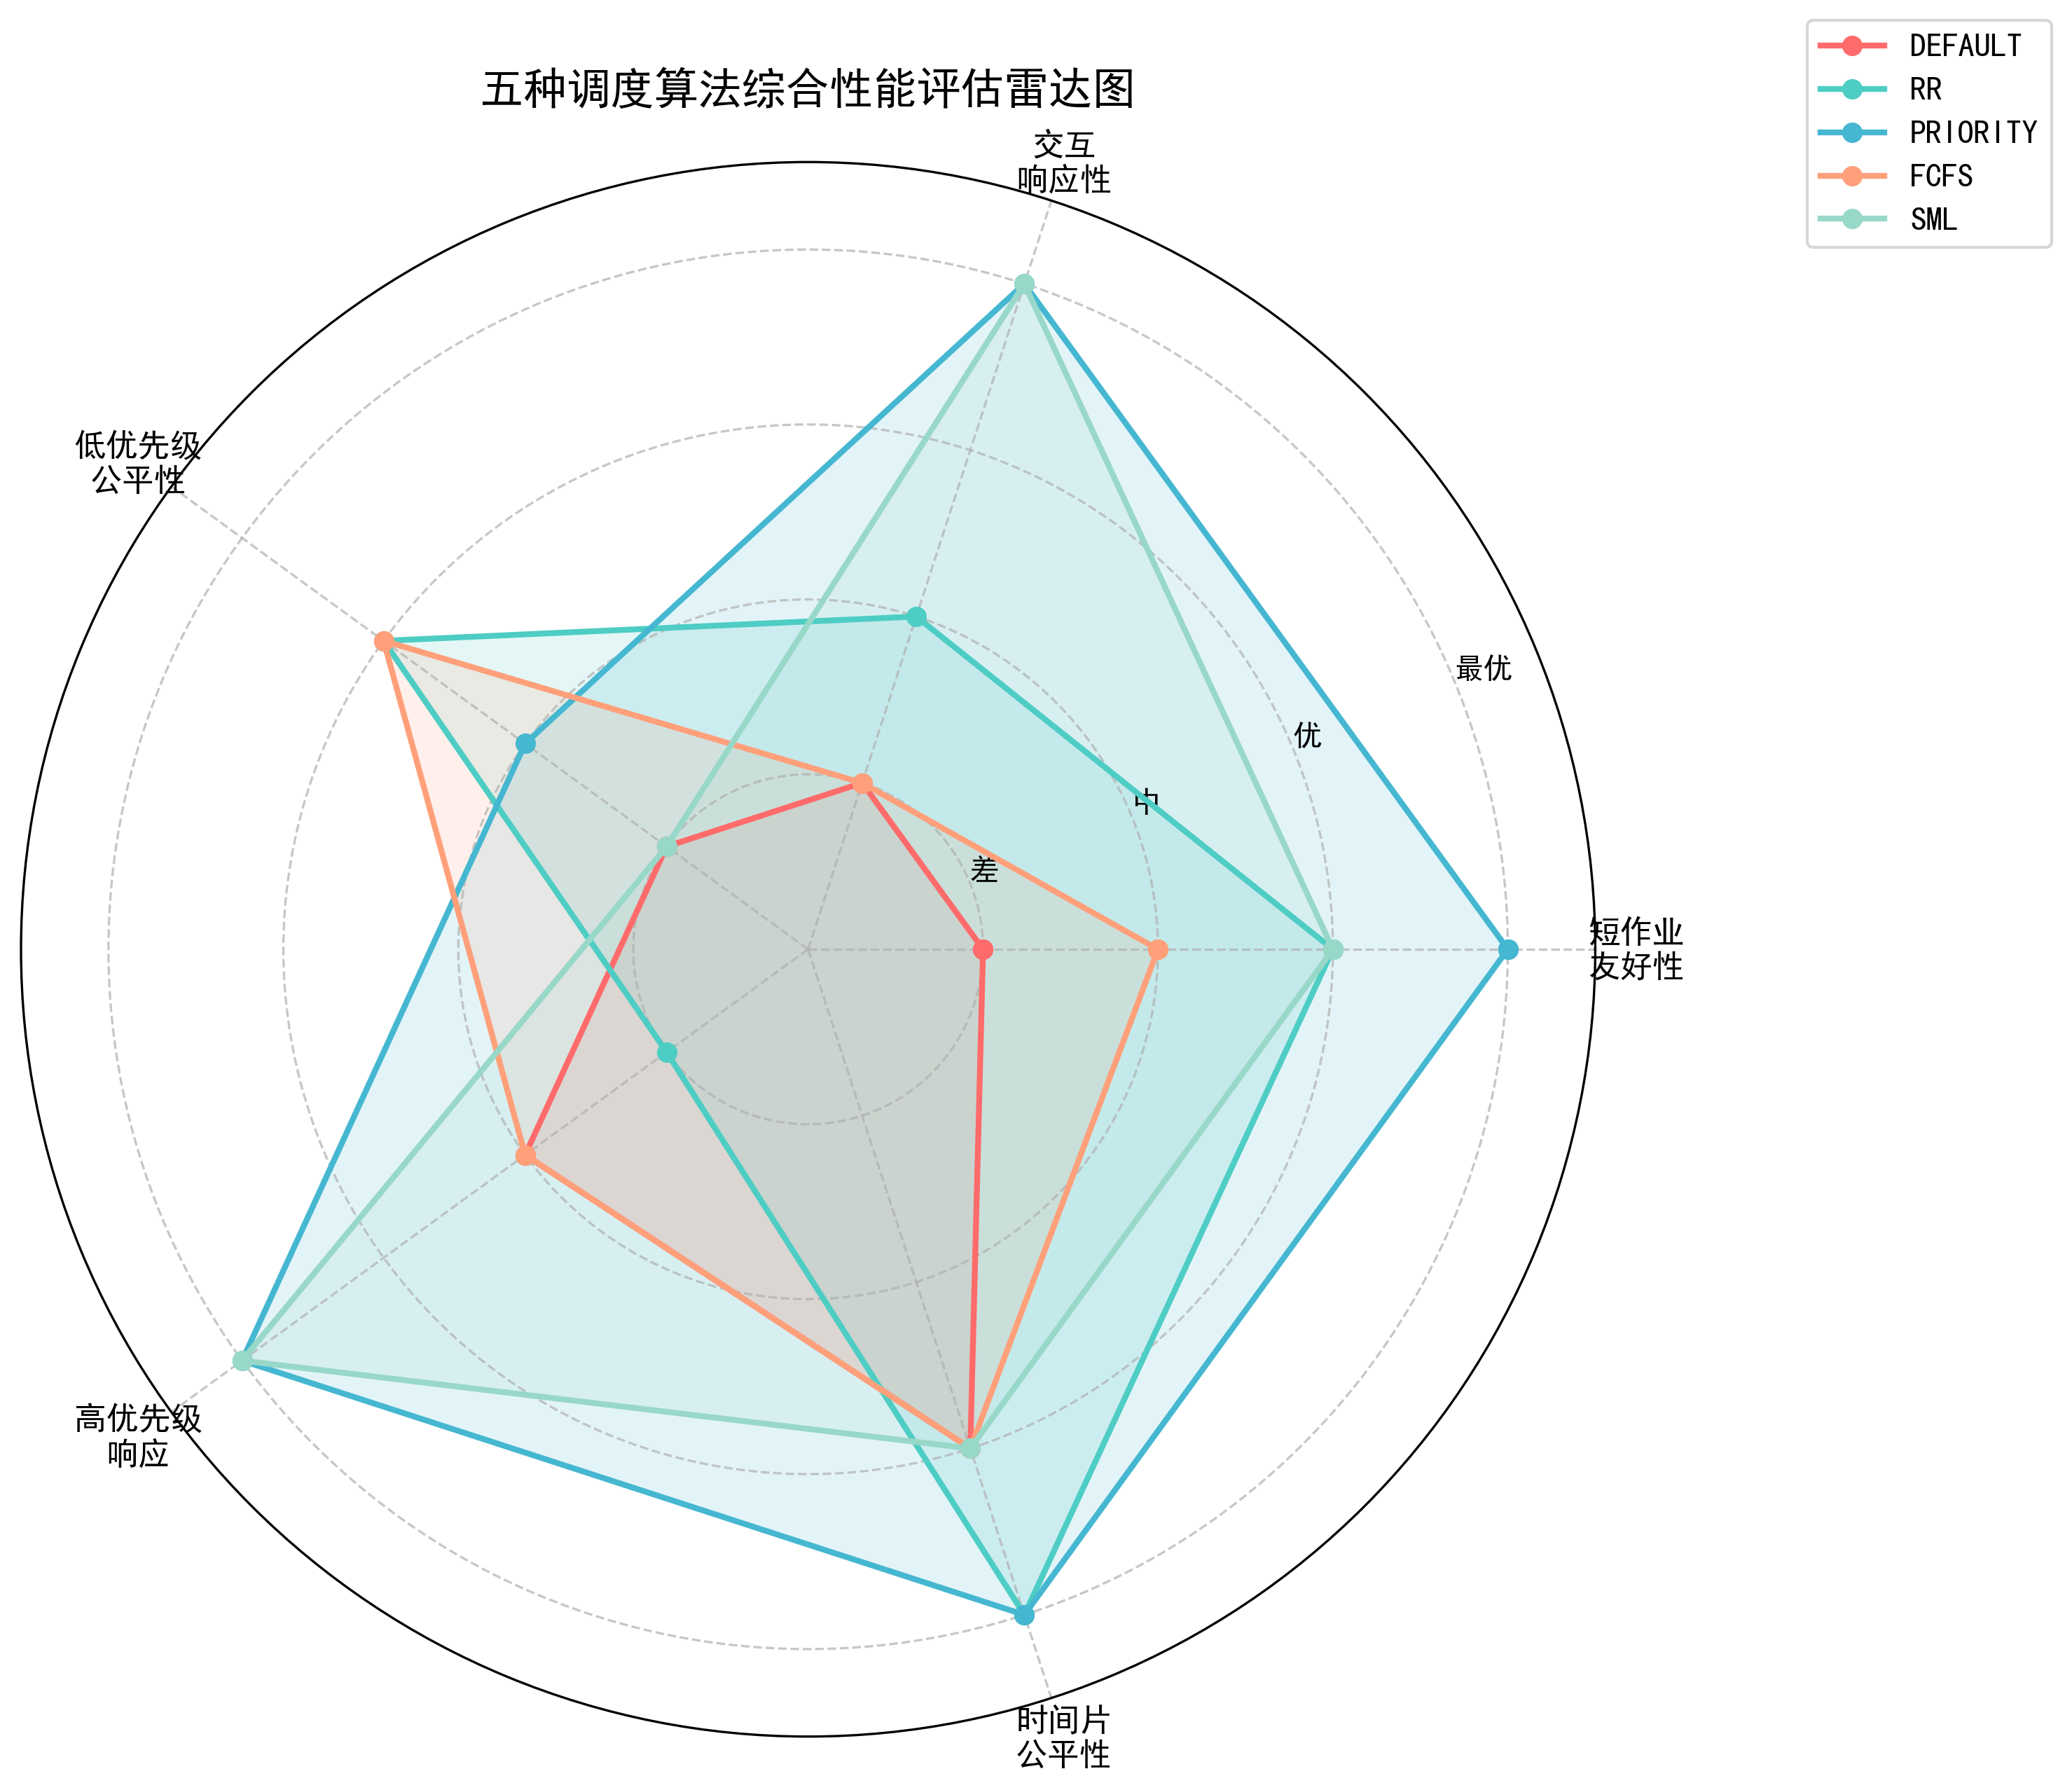
\includegraphics[width=0.6\textwidth]{img3/overall_performance_radar.png}
    	\caption{五种调度算法综合性能评估雷达图}
    	\label{fig:overall_radar}
    \end{figure}
    
    雷达图以五个维度全面评估各调度器的性能特征。PRIORITY调度器的覆盖面积最大，在短作业友好性、交互响应性和高优先级响应三个维度都达到最优，但在低优先级公平性上有所不足。RR调度器的图形较为均衡，在时间片公平性上表现最佳，适合需要公平调度的场景。SML综合了优先级和轮转的优点，在交互响应性和高优先级响应上达到最优。DEFAULT调度器在所有维度上表现平庸。FCFS在低优先级公平性上表现不错，但交互响应性较差。该图直观展示了"没有万能调度算法"的核心观点——应根据具体应用场景选择合适的调度策略。
    
    \section{实验中遇到的问题及解决方案}
    
    在本次实验过程中，遇到了多个技术问题。通过分析和调试，逐一找到了问题的根源并予以解决。以下是主要问题的记录与分析。
        
    \subsection{问题1：运行 scheduler\_test 时磁盘块耗尽}
    
    \textbf{现象：}运行 \texttt{scheduler\_test} 测试程序时，内核 panic：\texttt{"balloc: out of blocks"}
    
    \textbf{原因分析：}xv6 文件系统默认只有 1000 个块（约 500KB）。测试程序需要创建多个子进程，每个进程都会进行文件 IO 操作，加上结果输出文件的写入，很快就耗尽了磁盘空间。
    
    \textbf{解决方案：}修改 \texttt{param.h} 中的文件系统大小常量：
    \begin{codeblock}
	\#define FSSIZE 10000  // 从 1000 增加到 10000
    \end{codeblock}
    
    \subsection{问题2：PRIORITY/SML 调度器交互响应测试表现异常}
    
    \textbf{现象：}在场景2测试中，PRIORITY 调度器下高优先级的交互型任务（优先级3）平均就绪时间反而高于低优先级的 CPU 背景任务（优先级18），与预期相反。
    
    这是由多个因素共同导致的：
    \begin{enumerate}
        \item \textbf{非抢占式调度}：PRIORITY 和 SML 调度器只在进程主动让出 CPU 时才重新调度。CPU 密集型任务没有 \texttt{yield/sleep/exit} 调用，会一直运行到完成。
        \item \textbf{setpriority 时机问题}：测试程序中，子进程在 \texttt{fork()} 后才执行 \texttt{setpriority()}。在此之前，其他 CPU 密集型进程可能已经开始运行并占用 CPU。
        \item \textbf{进程创建顺序}：测试按顺序先创建 CPU 背景任务，再创建交互型任务。当交互型任务被创建时，CPU 背景任务已在运行且不会主动让出。
    \end{enumerate}
    
    \textbf{解决方案：}实现抢占式优先级调度，在时钟中断时检查是否有更高优先级进程就绪。

    
    \section{实验结论}
    
    本实验通过在 xv6 内核中实现并对比轮转（RR）、优先级（Priority）、先来先服务（FCFS）和静态多级队列（SML）四种调度算法，结合 \texttt{test\_scheduler.c} 构造的四个典型测试场景，深入分析了不同调度策略对系统性能的影响。
    
    实验数据表明，没有一种单一的简单调度算法能在所有场景下胜出。各算法的特性及适用场景总结如下：
    
    \begin{table}[H]
        \centering
        \caption{调度算法特性与适用场景分析}
        \begin{tabular}{|p{2.5cm}|p{4cm}|p{4cm}|p{3.5cm}|}
            \hline
            \textbf{调度算法} & \textbf{优势} & \textbf{劣势} & \textbf{适用场景} \\ \hline
            \textbf{FCFS} & 实现简单，无进程切换开销 & 严重的车队效应，短作业等待时间长，交互体验差 & 批处理系统，后台计算任务 \\ \hline
            \textbf{RR (轮转)} & 响应时间短，公平性好（方差小），防止饥饿 & 频繁切换开销大，未区分进程重要性，关键任务得不到优先处理 & 分时系统，多用户交互环境 \\ \hline
            \textbf{Priority} & 关键任务响应极快，支持不同服务等级 & 低优先级进程可能"饥饿"，优先级反转风险 & 实时系统，区分用户等级的系统 \\ \hline
            \textbf{SML (多级队列)} & 结合了响应性和灵活性，兼顾多种需求 & 静态队列配置死板，低优先级队列仍可能饥饿 & 复杂的通用操作系统 \\ \hline
        \end{tabular}
    \end{table}
    
    \subsection{从实验走向现代调度：完全公平调度 (CFS)}
    
    通过实验我们发现，传统的调度算法往往陷入"公平性"与"交互性"的博弈中：
    \begin{itemize}
        \item RR 追求绝对的时间片公平，却牺牲了重要进程的优先权；
        \item Priority 追求重要性优先，却带来了严重的饥饿和不公平问题；
        \item SML 虽然试图折中，但静态的队列划分依然不够灵活，难以应对瞬息万变的负载。
    \end{itemize}
    
    这正是现代 Linux 内核抛弃这些传统算法的原因。为了同时解决上述问题，Linux 2.6.23 引入了 完全公平调度器（Completely Fair Scheduler, CFS）。
    
    CFS不再使用离散的时间片和静态优先级，而是基于\textbf{虚拟运行时间 (vruntime)} 的概念。它通过红黑树结构动态维护进程队列，每次总是选择 vruntime 最小的进程运行。这种设计带来了质的飞跃：
    \begin{enumerate}
        \item \textbf{动态公平}：不需要复杂的时间片计算，vruntime 自动体现了进程占用 CPU 的"不公平程度"，调度器只需不断补偿"最不公平"的进程。
        \item \textbf{平滑优先级}：优先级被转化为权重，影响 vruntime 的增长速度。高优先级进程 vruntime 涨得慢，从而获得更多 CPU 时间，但不会像传统 Priority 那样完全饿死低优先级进程。
        \item \textbf{交互优化}：睡眠的交互进程唤醒时 vruntime 较小，能立即抢占 CPU，天然保证了低延迟。
    \end{enumerate}
    
        \begin{figure}[H]
    	\centering
    	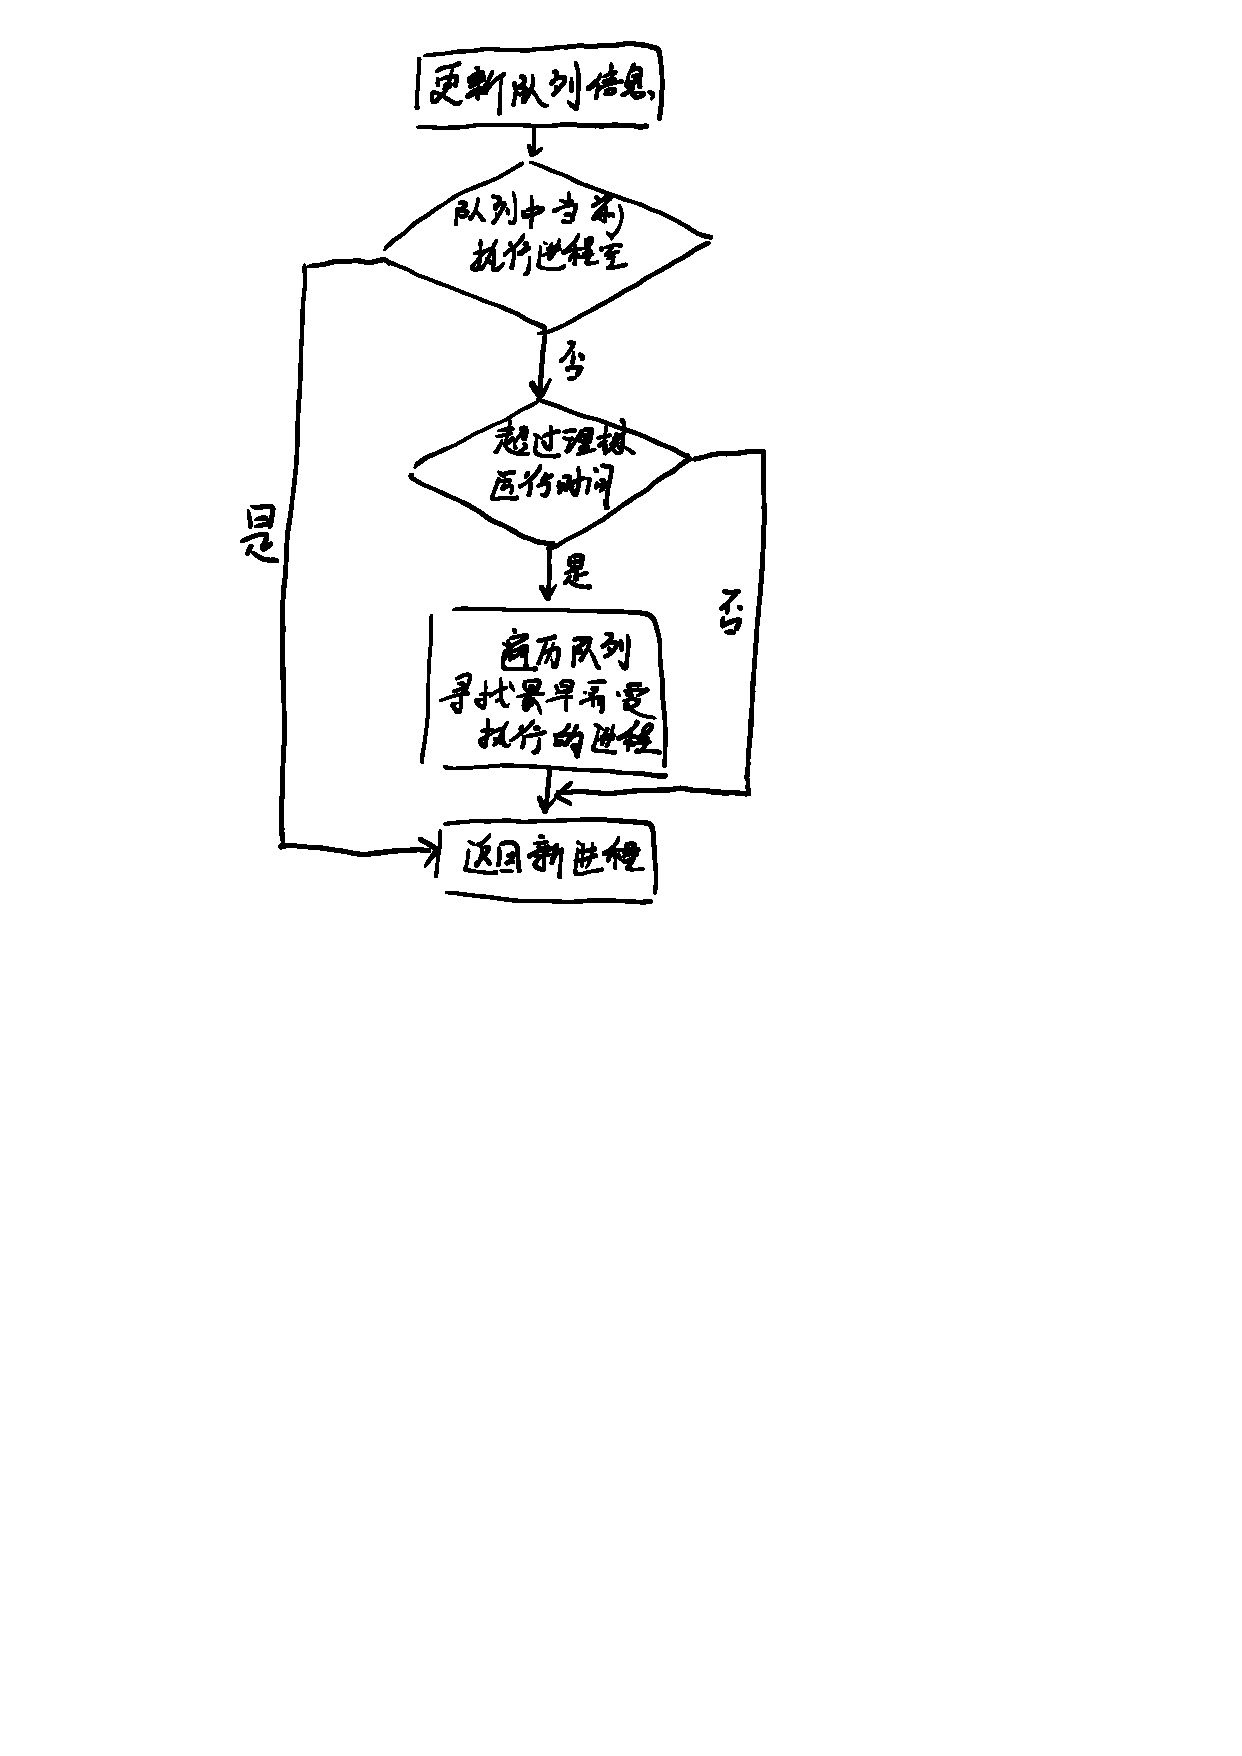
\includegraphics[width=0.45\textwidth]{img3/CFS.pdf}
    	\caption{完全公平调度算法大概流程图}
    	\label{fig:cfs}
    \end{figure}
    
    本次实验实现的算法是操作系统调度的基石，而理解它们的缺陷，正是理解 CFS 等现代复杂调度算法设计哲学的关键一把钥匙。

    
    \section{实验心得}
    
    这次实验让我对操作系统调度有了更深刻的认识。
    
    我深刻体会到了调度算法的选择对系统行为的深远影响。在实现和测试不同调度算法的过程中，我发现看似简单的调度决策实际上涉及到响应时间、吞吐量、公平性等多个相互制约的因素。例如，优先级调度虽然能让高优先级进程快速响应，但如果不加限制，低优先级进程可能永远得不到执行机会，这就是所谓的饥饿问题。
    
    此外，设计可扩展的调度框架让我对软件工程中的抽象和模块化有了新的理解。通过使用函数指针数组，我实现了调度算法的即插即用，这种设计使得添加新算法变得非常简单。这个经验让我意识到，好的架构设计能够极大地降低后续开发和维护的成本。
   
    
    \newpage
    \subsection{附录A：调度器框架与数据结构}
    
    \subsubsection{A.1 就绪队列数据结构}
    
    \begin{codeblock}{proc.c - 队列与堆结构定义}
// 通用队列结构单元
struct procqueue {
    struct proc *head;
    struct proc *tail;
};

// FCFS/RR 队列（1个）
struct procqueue fcfsQueue;

// Priority 最小堆，优先级越小越靠前
struct priorityHeap {
    struct proc *procs[NPROC]; // 堆数组
    int size;                  // 当前堆大小
} pHeap;

// SML 队列（3个：0=高优先级1-7, 1=中优先级8-14, 2=低优先级15-20）
struct procqueue smlQueues[3];
    \end{codeblock}
    
    \subsubsection{A.2 队列操作函数}
    
    \begin{codeblock}{enqueue/dequeue 实现}
// 入队：将进程添加到队列尾部
void enqueue(struct procqueue *q, struct proc *p) {
    p->next = 0;
    if (q->tail == 0) {
        q->head = q->tail = p;
    } else {
        q->tail->next = p;
        q->tail = p;
    }
}

// 出队：从队列头部取出进程
struct proc *dequeue(struct procqueue *q) {
    struct proc *p = q->head;
    if (p == 0) return 0;
    q->head = p->next;
    if (q->head == 0) {
        q->tail = 0;
    }
    p->next = 0;
    return p;
}
    \end{codeblock}
    
    \subsubsection{A.3 统一入队函数}
    
    \begin{codeblock}{addToReadyQueues 实现}
// 统一入队函数：进程变为 RUNNABLE 时调用
// 根据当前激活的调度器，只添加到对应的队列
extern int schedSelected; // 来自 sdh.h，表示当前调度器类型

void addToReadyQueues(struct proc *p) {
    switch (schedSelected) {
    case 0: // DEFAULT
    case 2: // FCFS
    case 3: // RR
        enqueue(&fcfsQueue, p);
        break;
    case 1: // PRIORITY - 使用最小堆
        heapInsert(p);
        break;
    case 4: // SML
        if (p->priority >= 1 && p->priority <= 7) {
            enqueue(&smlQueues[0], p);
        } else if (p->priority >= 8 && p->priority <= 14) {
            enqueue(&smlQueues[1], p);
        } else {
            enqueue(&smlQueues[2], p);
        }
        break;
    default:
        enqueue(&fcfsQueue, p);
        break;
    }
}
    \end{codeblock}
    
    \subsection{附录B：调度算法实现}
    
    \subsubsection{B.1 优先级调度器（Priority Scheduler）}
    
    \begin{codeblock}{priorityScheduler 实现}
// 优先级调度器：遍历进程表，选择优先级最高（数值最小）的就绪进程
// 时间复杂度 O(n)，但能实时反映优先级变化
struct proc *priorityScheduler() {
    struct proc *p, *best = 0;
    for (p = ptable.proc; p < &ptable.proc[NPROC]; p++) {
        if (p->state == RUNNABLE) {
            if (best == 0 || p->priority < best->priority)
                best = p;
        }
    }
    if (best != 0) best->state = RUNNING;
    return best;
}
    \end{codeblock}
    
    \subsubsection{B.2 先来先服务调度器（FCFS）}
    
    \begin{codeblock}{fcfsScheduler 实现}
// 先来先服务调度器：从队列头部取出进程
// 非抢占式，进程运行直到主动让出CPU
struct proc *fcfsScheduler() {
    return dequeue(&fcfsQueue);
}
    \end{codeblock}
    
    \subsubsection{B.3 轮转调度器（Round Robin）}
    
    \begin{codeblock}{rrScheduler 实现}
// 轮转调度器：从FCFS队列取出，调度后由yield重新入队尾
// 与FCFS共用队列，但在trap.c中会被时钟中断抢占
struct proc *rrScheduler() {
    return dequeue(&fcfsQueue);
}
    \end{codeblock}
    
    \subsubsection{B.4 静态多级队列调度器（SML）}
    
    \begin{codeblock}{smlScheduler 实现}
// 静态多级队列调度器：依次从高、中、低优先级队列出队
// 高优先级队列优先，同级别内轮转（FCFS）
// 时间复杂度 O(1)
struct proc *smlScheduler() {
    struct proc *p;
    
    // 优先从高优先级队列出队
    p = dequeue(&smlQueues[0]);
    if (p != 0) return p;
    
    // 高优先级队列空，尝试中优先级队列
    p = dequeue(&smlQueues[1]);
    if (p != 0) return p;
    
    // 中优先级队列也空，尝试低优先级队列
    return dequeue(&smlQueues[2]);
}
    \end{codeblock}
    
    \subsection{附录C：调度器框架}
    
    \subsubsection{C.1 调度器选择机制（sdh.c）}
    
    \begin{codeblock}{sdh.c - 调度器函数指针数组}
#include "types.h"
#include "defs.h"
#include "proc.h"
#include "sdh.h"

// 全局调度器ID（默认为0）
int schedSelected = 0;

// 调度算法函数指针数组
struct proc *(*schedulerFunction[5])(void);

// 当前激活的调度函数指针
struct proc *(*ready_process)(void);

// 初始化调度器
void initScheduler(void) {
    schedulerFunction[0] = defaultScheduler;  // DEFAULT
    schedulerFunction[1] = priorityScheduler; // PRIORITY
    schedulerFunction[2] = fcfsScheduler;     // FCFS
    schedulerFunction[3] = rrScheduler;       // RR
    schedulerFunction[4] = smlScheduler;      // SML
    
    ready_process = schedulerFunction[0];
}

// 切换调度器
int setscheduler(int schedId) {
    if (schedId < 0 || schedId > 4) return -1;
    schedSelected = schedId;
    ready_process = schedulerFunction[schedId];
    return 0;
}
    \end{codeblock}
    
    \subsubsection{C.2 调度器主循环（scheduler函数）}
    
    \begin{codeblock}{proc.c - scheduler函数}
// scheduler - 调度器主循环函数
// 功能：操作系统的核心调度循环，负责选择并切换到下一个要执行的进程
// 说明：此函数永不返回，每个CPU核心启动后会一直在此循环中运行
void scheduler(void) {
    struct proc *p;
    struct cpu *c = mycpu();
    c->proc = 0;
    
    for (;;) {
        // 步骤1：启用中断，防止死锁
        sti();
        
        // 步骤2：获取进程表锁
        acquire(&ptable.lock);
        
        // 步骤3：调用当前选定的调度算法选择下一个进程
        acquire(&schedulerlock);
        p = (*ready_process)();
        release(&schedulerlock);
        
        // 步骤4：如果找到了就绪进程，则进行上下文切换
        if (p != 0) {
            c->proc = p;
            switchuvm(p);           // 切换到进程的页表
            p->state = RUNNING;
            swtch(&(c->scheduler), p->context);  // 上下文切换
            switchkvm();            // 恢复内核页表
            c->proc = 0;
        }
        
        // 步骤5：释放进程表锁
        release(&ptable.lock);
    }
}
    \end{codeblock}
    
    \subsubsection{C.3 进程让出CPU（yield函数）}
    
    \begin{codeblock}{proc.c - yield函数}
// yield - 进程主动放弃CPU资源
// 用于实现轮转调度的时间片机制
void yield(void) {
    acquire(&ptable.lock);
    struct proc *curp = myproc();
    curp->state = RUNNABLE;
    addToReadyQueues(curp);  // 重新加入就绪队列
    sched();                  // 切换到调度器
    release(&ptable.lock);
}
    \end{codeblock}
    
    \subsection{附录D：时钟中断与进程统计}
    
    \subsubsection{D.1 时钟中断处理（trap.c）}
    
    \begin{codeblock}{trap.c - 时钟中断处理}
void trap(struct trapframe *tf) {
    // ... 省略系统调用处理 ...
    
    switch (tf->trapno) {
    case T_IRQ0 + IRQ_TIMER:  // 时钟中断
        if (cpuid() == 0) {
            acquire(&tickslock);
            ticks++;                  // 增加全局时钟计数
            update_statistics();      // 更新进程时间统计
            wakeup(&ticks);           // 唤醒等待时钟的进程
            release(&tickslock);
        }
        lapiceoi();
        break;
    // ... 省略其他中断处理 ...
    }
    
    // 抢占式调度：时间片用完就让出CPU
    if (myproc() && myproc()->state == RUNNING &&
        tf->trapno == T_IRQ0 + IRQ_TIMER) {
        yield();  // 无条件让出CPU，由调度器决定下一个进程
    }
}
    \end{codeblock}
    
    \subsubsection{D.2 进程时间统计更新}
    
    \begin{codeblock}{proc.c - update\_statistics函数}
// update_statistics - 更新所有进程的时间统计
// 每个时钟中断调用一次
void update_statistics(void) {
    struct proc *p;
    acquire(&ptable.lock);
    
    for (p = ptable.proc; p < &ptable.proc[NPROC]; p++) {
        switch (p->state) {
        case RUNNING:
            p->rutime++;   // 运行时间 +1
            break;
        case RUNNABLE:
            p->retime++;   // 就绪等待时间 +1
            break;
        case SLEEPING:
            p->stime++;    // 睡眠时间 +1
            break;
        default:
            break;
        }
    }
    
    release(&ptable.lock);
}
    \end{codeblock}
    
    \subsubsection{D.3 wait2系统调用}
    
    \begin{codeblock}{proc.c - wait2函数}
// wait2 - wait的增强版，返回子进程的时间统计信息
int wait2(int *retime, int *rutime, int *stime) {
    struct proc *p;
    int havekids, pid;
    
    acquire(&ptable.lock);
    for (;;) {
        havekids = 0;
        for (p = ptable.proc; p < &ptable.proc[NPROC]; p++) {
            if (p->parent != myproc()) continue;
            havekids = 1;
            
            if (p->state == ZOMBIE) {
                // 收集时间统计信息
                *retime = p->retime;  // 就绪等待时间
                *rutime = p->rutime;  // 实际运行时间
                *stime = p->stime;    // 睡眠时间
                
                pid = p->pid;
                // 释放进程资源...
                kfree(p->kstack);
                p->kstack = 0;
                freevm(p->pgdir);
                p->state = UNUSED;
                // 清零统计字段...
                
                release(&ptable.lock);
                return pid;
            }
        }
        
        if (!havekids || myproc()->killed) {
            release(&ptable.lock);
            return -1;
        }
        
        sleep(myproc(), &ptable.lock);
    }
}
    \end{codeblock}
    
% ==========================================
% 附录：完整实验结果
% ==========================================
\section{附录：完整实验结果}\label{appendix:full-results}

% ============================================================
% 场景1：纯CPU长短作业（车队效应测试）
% ============================================================
\subsection{场景1：纯CPU长短作业（车队效应测试）}

\begin{table}[H]
	\centering
	\caption{场景1 - DEFAULT调度器测试结果}
	\begin{tabular}{cccrrr}
		\toprule
		\textbf{PID} & \textbf{优先级} & \textbf{类型} & \textbf{就绪时间} & \textbf{运行时间} & \textbf{周转时间} \\
		\midrule
		4 & 10 & 长作业 & 24 & 219 & 243 \\
		5 & 10 & 长作业 & 263 & 218 & 481 \\
		6 & 10 & 短作业 & 460 & 22 & 550 \\
		7 & 10 & 短作业 & 471 & 22 & 623 \\
		8 & 10 & 中作业 & 478 & 75 & 621 \\
		9 & 10 & 中作业 & 538 & 75 & 627 \\
		\midrule
		\multicolumn{3}{c}{长作业平均} & 143 & 218 & 362 \\
		\multicolumn{3}{c}{短作业平均} & 465 & 22 & 487 \\
		\multicolumn{3}{c}{中作业平均} & 508 & 75 & 583 \\
		\bottomrule
	\end{tabular}
\end{table}

\begin{table}[H]
	\centering
	\caption{场景1 - RR(轮转)调度器测试结果}
	\begin{tabular}{cccrrr}
		\toprule
		\textbf{PID} & \textbf{优先级} & \textbf{类型} & \textbf{就绪时间} & \textbf{运行时间} & \textbf{周转时间} \\
		\midrule
		30 & 10 & 短作业 & 102 & 21 & 123 \\
		31 & 10 & 短作业 & 147 & 22 & 382 \\
		32 & 10 & 中作业 & 266 & 74 & 370 \\
		33 & 10 & 中作业 & 266 & 72 & 370 \\
		28 & 10 & 长作业 & 407 & 225 & 639 \\
		29 & 10 & 长作业 & 408 & 216 & 637 \\
		\midrule
		\multicolumn{3}{c}{长作业平均} & 407 & 220 & 628 \\
		\multicolumn{3}{c}{短作业平均} & 124 & 21 & 146 \\
		\multicolumn{3}{c}{中作业平均} & 266 & 73 & 339 \\
		\bottomrule
	\end{tabular}
\end{table}

\begin{table}[H]
	\centering
	\caption{场景1 - PRIORITY调度器测试结果}
	\begin{tabular}{cccrrr}
		\toprule
		\textbf{PID} & \textbf{优先级} & \textbf{类型} & \textbf{就绪时间} & \textbf{运行时间} & \textbf{周转时间} \\
		\midrule
		52 & 10 & 长作业 & 215 & 217 & 432 \\
		53 & 10 & 长作业 & 215 & 214 & 429 \\
		54 & 10 & 短作业 & 24 & 21 & 45 \\
		55 & 10 & 短作业 & 21 & 22 & 43 \\
		56 & 10 & 中作业 & 73 & 71 & 144 \\
		57 & 10 & 中作业 & 73 & 74 & 147 \\
		\midrule
		\multicolumn{3}{c}{长作业平均} & 215 & 215 & 430 \\
		\multicolumn{3}{c}{短作业平均} & 22 & 21 & 44 \\
		\multicolumn{3}{c}{中作业平均} & 73 & 72 & 145 \\
		\bottomrule
	\end{tabular}
\end{table}

\begin{table}[H]
	\centering
	\caption{场景1 - FCFS调度器测试结果}
	\begin{tabular}{cccrrr}
		\toprule
		\textbf{PID} & \textbf{优先级} & \textbf{类型} & \textbf{就绪时间} & \textbf{运行时间} & \textbf{周转时间} \\
		\midrule
		76 & 10 & 长作业 & 1 & 214 & 215 \\
		77 & 10 & 长作业 & 214 & 214 & 428 \\
		78 & 10 & 短作业 & 0 & 22 & 22 \\
		79 & 10 & 短作业 & 22 & 22 & 44 \\
		80 & 10 & 中作业 & 1 & 71 & 72 \\
		81 & 10 & 中作业 & 72 & 72 & 144 \\
		\midrule
		\multicolumn{3}{c}{长作业平均} & 107 & 214 & 321 \\
		\multicolumn{3}{c}{短作业平均} & 11 & 22 & 33 \\
		\multicolumn{3}{c}{中作业平均} & 36 & 71 & 108 \\
		\bottomrule
	\end{tabular}
\end{table}

\begin{table}[H]
	\centering
	\caption{场景1 - SML(多级队列)调度器测试结果}
	\begin{tabular}{cccrrr}
		\toprule
		\textbf{PID} & \textbf{优先级} & \textbf{类型} & \textbf{就绪时间} & \textbf{运行时间} & \textbf{周转时间} \\
		\midrule
		102 & 10 & 短作业 & 106 & 21 & 134 \\
		103 & 10 & 短作业 & 110 & 22 & 134 \\
		104 & 10 & 中作业 & 287 & 72 & 515 \\
		100 & 10 & 长作业 & 404 & 227 & 631 \\
		101 & 10 & 长作业 & 407 & 216 & 631 \\
		105 & 10 & 中作业 & 286 & 71 & 515 \\
		\midrule
		\multicolumn{3}{c}{长作业平均} & 405 & 221 & 627 \\
		\multicolumn{3}{c}{短作业平均} & 108 & 21 & 129 \\
		\multicolumn{3}{c}{中作业平均} & 286 & 71 & 358 \\
		\bottomrule
	\end{tabular}
\end{table}

% ============================================================
% 场景2：交互型vs背景任务
% ============================================================
\subsection{场景2：交互型vs背景任务}

\begin{table}[H]
	\centering
	\caption{场景2 - DEFAULT调度器测试结果}
	\begin{tabular}{cccrrrr}
		\toprule
		\textbf{PID} & \textbf{优先级} & \textbf{类型} & \textbf{就绪时间} & \textbf{运行时间} & \textbf{休眠时间} & \textbf{周转时间} \\
		\midrule
		10 & 18 & CPU背景 & 9 & 217 & 225 & 451 \\
		11 & 18 & CPU背景 & 228 & 215 & 9 & 452 \\
		12 & 3 & 交互型 & 440 & 80 & 189 & 709 \\
		13 & 3 & 交互型 & 514 & 81 & 121 & 716 \\
		14 & 12 & IO背景 & 593 & 45 & 222 & 860 \\
		15 & 12 & IO背景 & 265 & 46 & 556 & 867 \\
		\midrule
		\multicolumn{3}{c}{交互型平均} & 477 & 80 & 155 & 712 \\
		\multicolumn{3}{c}{CPU背景平均} & 118 & 216 & 0 & 334 \\
		\multicolumn{3}{c}{IO背景平均} & 429 & 45 & 389 & 863 \\
		\bottomrule
	\end{tabular}
\end{table}

\begin{table}[H]
	\centering
	\caption{场景2 - RR(轮转)调度器测试结果}
	\begin{tabular}{cccrrrr}
		\toprule
		\textbf{PID} & \textbf{优先级} & \textbf{类型} & \textbf{就绪时间} & \textbf{运行时间} & \textbf{休眠时间} & \textbf{周转时间} \\
		\midrule
		36 & 3 & 交互型 & 398 & 81 & 86 & 565 \\
		37 & 3 & 交互型 & 398 & 81 & 86 & 565 \\
		34 & 18 & CPU背景 & 447 & 236 & 6 & 689 \\
		35 & 18 & CPU背景 & 451 & 215 & 23 & 689 \\
		38 & 12 & IO背景 & 458 & 44 & 275 & 777 \\
		39 & 12 & IO背景 & 455 & 45 & 301 & 801 \\
		\midrule
		\multicolumn{3}{c}{交互型平均} & 398 & 81 & 86 & 565 \\
		\multicolumn{3}{c}{CPU背景平均} & 449 & 225 & 0 & 674 \\
		\multicolumn{3}{c}{IO背景平均} & 456 & 44 & 288 & 789 \\
		\bottomrule
	\end{tabular}
\end{table}

\begin{table}[H]
	\centering
	\caption{场景2 - PRIORITY调度器测试结果}
	\begin{tabular}{cccrrrr}
		\toprule
		\textbf{PID} & \textbf{优先级} & \textbf{类型} & \textbf{就绪时间} & \textbf{运行时间} & \textbf{休眠时间} & \textbf{周转时间} \\
		\midrule
		60 & 3 & 交互型 & 73 & 80 & 200 & 353 \\
		61 & 3 & 交互型 & 72 & 81 & 200 & 353 \\
		62 & 12 & IO背景 & 230 & 41 & 396 & 667 \\
		63 & 12 & IO背景 & 225 & 40 & 448 & 713 \\
		58 & 18 & CPU背景 & 475 & 236 & 10 & 721 \\
		59 & 18 & CPU背景 & 480 & 232 & 13 & 725 \\
		\midrule
		\multicolumn{3}{c}{交互型平均} & 72 & 80 & 200 & 353 \\
		\multicolumn{3}{c}{CPU背景平均} & 477 & 234 & 0 & 711 \\
		\multicolumn{3}{c}{IO背景平均} & 227 & 40 & 422 & 690 \\
		\bottomrule
	\end{tabular}
\end{table}

\begin{table}[H]
	\centering
	\caption{场景2 - FCFS调度器测试结果}
	\begin{tabular}{cccrrrr}
		\toprule
		\textbf{PID} & \textbf{优先级} & \textbf{类型} & \textbf{就绪时间} & \textbf{运行时间} & \textbf{休眠时间} & \textbf{周转时间} \\
		\midrule
		82 & 18 & CPU背景 & 1 & 215 & 0 & 216 \\
		83 & 18 & CPU背景 & 216 & 214 & 0 & 430 \\
		84 & 3 & 交互型 & 523 & 80 & 108 & 711 \\
		85 & 3 & 交互型 & 538 & 84 & 96 & 718 \\
		86 & 12 & IO背景 & 592 & 41 & 222 & 855 \\
		87 & 12 & IO背景 & 597 & 41 & 226 & 864 \\
		\midrule
		\multicolumn{3}{c}{交互型平均} & 530 & 82 & 102 & 714 \\
		\multicolumn{3}{c}{CPU背景平均} & 108 & 214 & 0 & 323 \\
		\multicolumn{3}{c}{IO背景平均} & 594 & 41 & 224 & 859 \\
		\bottomrule
	\end{tabular}
\end{table}

\begin{table}[H]
	\centering
	\caption{场景2 - SML(多级队列)调度器测试结果}
	\begin{tabular}{cccrrrr}
		\toprule
		\textbf{PID} & \textbf{优先级} & \textbf{类型} & \textbf{就绪时间} & \textbf{运行时间} & \textbf{休眠时间} & \textbf{周转时间} \\
		\midrule
		108 & 3 & 交互型 & 73 & 80 & 200 & 353 \\
		109 & 3 & 交互型 & 77 & 80 & 196 & 353 \\
		110 & 12 & IO背景 & 240 & 40 & 367 & 647 \\
		106 & 18 & CPU背景 & 477 & 239 & 0 & 716 \\
		107 & 18 & CPU背景 & 480 & 233 & 9 & 722 \\
		111 & 12 & IO背景 & 223 & 41 & 467 & 731 \\
		\midrule
		\multicolumn{3}{c}{交互型平均} & 75 & 80 & 198 & 353 \\
		\multicolumn{3}{c}{CPU背景平均} & 478 & 236 & 0 & 714 \\
		\multicolumn{3}{c}{IO背景平均} & 231 & 40 & 417 & 689 \\
		\bottomrule
	\end{tabular}
\end{table}

% ============================================================
% 场景3：优先级饥饿测试
% ============================================================
\subsection{场景3：优先级饥饿测试}

\begin{table}[H]
	\centering
	\caption{场景3 - DEFAULT调度器测试结果}
	\begin{tabular}{cccrrr}
		\toprule
		\textbf{PID} & \textbf{优先级} & \textbf{优先级组} & \textbf{就绪时间} & \textbf{运行时间} & \textbf{周转时间} \\
		\midrule
		16 & 1 & 高优先级 & 40 & 436 & 476 \\
		17 & 10 & 中优先级 & 481 & 111 & 592 \\
		18 & 10 & 中优先级 & 586 & 110 & 696 \\
		19 & 10 & 中优先级 & 688 & 110 & 798 \\
		20 & 19 & 低优先级 & 780 & 111 & 891 \\
		21 & 19 & 低优先级 & 880 & 112 & 992 \\
		\midrule
		\multicolumn{3}{c}{高优平均} & 40 & 436 & 476 \\
		\multicolumn{3}{c}{中优平均} & 585 & 110 & 695 \\
		\multicolumn{3}{c}{低优平均} & 830 & 111 & 941 \\
		\bottomrule
	\end{tabular}
\end{table}

\begin{table}[H]
	\centering
	\caption{场景3 - RR(轮转)调度器测试结果}
	\begin{tabular}{cccrrr}
		\toprule
		\textbf{PID} & \textbf{优先级} & \textbf{优先级组} & \textbf{就绪时间} & \textbf{运行时间} & \textbf{周转时间} \\
		\midrule
		41 & 10 & 中优先级 & 539 & 108 & 647 \\
		42 & 10 & 中优先级 & 537 & 107 & 644 \\
		43 & 10 & 中优先级 & 537 & 107 & 644 \\
		44 & 19 & 低优先级 & 540 & 108 & 648 \\
		45 & 19 & 低优先级 & 584 & 108 & 933 \\
		40 & 1 & 高优先级 & 540 & 446 & 988 \\
		\midrule
		\multicolumn{3}{c}{高优平均} & 540 & 446 & 986 \\
		\multicolumn{3}{c}{中优平均} & 537 & 107 & 645 \\
		\multicolumn{3}{c}{低优平均} & 562 & 108 & 670 \\
		\bottomrule
	\end{tabular}
\end{table}

\begin{table}[H]
	\centering
	\caption{场景3 - PRIORITY调度器测试结果}
	\begin{tabular}{cccrrr}
		\toprule
		\textbf{PID} & \textbf{优先级} & \textbf{优先级组} & \textbf{就绪时间} & \textbf{运行时间} & \textbf{周转时间} \\
		\midrule
		64 & 1 & 高优先级 & 1 & 427 & 428 \\
		66 & 10 & 中优先级 & 124 & 107 & 301 \\
		65 & 10 & 中优先级 & 554 & 107 & 805 \\
		67 & 10 & 中优先级 & 217 & 113 & 377 \\
		69 & 19 & 低优先级 & 409 & 112 & 521 \\
		68 & 19 & 低优先级 & 442 & 113 & 556 \\
		\midrule
		\multicolumn{3}{c}{高优平均} & 1 & 427 & 428 \\
		\multicolumn{3}{c}{中优平均} & 298 & 109 & 407 \\
		\multicolumn{3}{c}{低优平均} & 425 & 112 & 538 \\
		\bottomrule
	\end{tabular}
\end{table}

\begin{table}[H]
	\centering
	\caption{场景3 - FCFS调度器测试结果}
	\begin{tabular}{cccrrr}
		\toprule
		\textbf{PID} & \textbf{优先级} & \textbf{优先级组} & \textbf{就绪时间} & \textbf{运行时间} & \textbf{周转时间} \\
		\midrule
		88 & 1 & 高优先级 & 2 & 437 & 439 \\
		89 & 10 & 中优先级 & 439 & 108 & 547 \\
		90 & 10 & 中优先级 & 547 & 107 & 654 \\
		91 & 10 & 中优先级 & 654 & 109 & 763 \\
		92 & 19 & 低优先级 & 762 & 107 & 869 \\
		93 & 19 & 低优先级 & 869 & 108 & 977 \\
		\midrule
		\multicolumn{3}{c}{高优平均} & 2 & 437 & 439 \\
		\multicolumn{3}{c}{中优平均} & 546 & 108 & 654 \\
		\multicolumn{3}{c}{低优平均} & 815 & 107 & 923 \\
		\bottomrule
	\end{tabular}
\end{table}

\begin{table}[H]
	\centering
	\caption{场景3 - SML(多级队列)调度器测试结果}
	\begin{tabular}{cccrrr}
		\toprule
		\textbf{PID} & \textbf{优先级} & \textbf{优先级组} & \textbf{就绪时间} & \textbf{运行时间} & \textbf{周转时间} \\
		\midrule
		112 & 1 & 高优先级 & 1 & 429 & 430 \\
		114 & 10 & 中优先级 & 648 & 108 & 756 \\
		115 & 10 & 中优先级 & 648 & 107 & 755 \\
		113 & 10 & 中优先级 & 647 & 113 & 899 \\
		116 & 19 & 低优先级 & 870 & 112 & 982 \\
		117 & 19 & 低优先级 & 871 & 114 & 989 \\
		\midrule
		\multicolumn{3}{c}{高优平均} & 1 & 429 & 430 \\
		\multicolumn{3}{c}{中优平均} & 647 & 109 & 757 \\
		\multicolumn{3}{c}{低优平均} & 870 & 113 & 983 \\
		\bottomrule
	\end{tabular}
\end{table}

% ============================================================
% 场景4：时间片公平性测试
% ============================================================
\subsection{场景4：时间片公平性测试}

\begin{table}[H]
	\centering
	\caption{场景4 - DEFAULT调度器测试结果}
	\begin{tabular}{ccrrr}
		\toprule
		\textbf{PID} & \textbf{优先级} & \textbf{就绪时间} & \textbf{运行时间} & \textbf{周转时间} \\
		\midrule
		22 & 10 & 10 & 109 & 119 \\
		23 & 10 & 132 & 110 & 242 \\
		24 & 10 & 250 & 109 & 359 \\
		25 & 10 & 355 & 110 & 465 \\
		26 & 10 & 455 & 112 & 567 \\
		27 & 10 & 550 & 111 & 661 \\
		\midrule
		\multicolumn{2}{c}{平均运行时间} & \multicolumn{3}{c}{110} \\
		\multicolumn{2}{c}{运行时间方差} & \multicolumn{3}{c}{\textbf{1}} \\
		\bottomrule
	\end{tabular}
\end{table}

\begin{table}[H]
	\centering
	\caption{场景4 - RR(轮转)调度器测试结果}
	\begin{tabular}{ccrrr}
		\toprule
		\textbf{PID} & \textbf{优先级} & \textbf{就绪时间} & \textbf{运行时间} & \textbf{周转时间} \\
		\midrule
		46 & 10 & 537 & 108 & 645 \\
		47 & 10 & 534 & 107 & 641 \\
		48 & 10 & 537 & 108 & 646 \\
		49 & 10 & 537 & 107 & 646 \\
		50 & 10 & 537 & 107 & 646 \\
		51 & 10 & 537 & 108 & 646 \\
		\midrule
		\multicolumn{2}{c}{平均运行时间} & \multicolumn{3}{c}{107} \\
		\multicolumn{2}{c}{运行时间方差} & \multicolumn{3}{c}{\textbf{0}} \\
		\bottomrule
	\end{tabular}
\end{table}

\begin{table}[H]
	\centering
	\caption{场景4 - PRIORITY调度器测试结果}
	\begin{tabular}{ccrrr}
		\toprule
		\textbf{PID} & \textbf{优先级} & \textbf{就绪时间} & \textbf{运行时间} & \textbf{周转时间} \\
		\midrule
		70 & 10 & 109 & 108 & 649 \\
		71 & 10 & 539 & 108 & 652 \\
		72 & 10 & 539 & 107 & 653 \\
		73 & 10 & 326 & 107 & 657 \\
		75 & 10 & 109 & 107 & 652 \\
		74 & 10 & 326 & 108 & 667 \\
		\midrule
		\multicolumn{2}{c}{平均运行时间} & \multicolumn{3}{c}{107} \\
		\multicolumn{2}{c}{运行时间方差} & \multicolumn{3}{c}{\textbf{0}} \\
		\bottomrule
	\end{tabular}
\end{table}

\begin{table}[H]
	\centering
	\caption{场景4 - FCFS调度器测试结果}
	\begin{tabular}{ccrrr}
		\toprule
		\textbf{PID} & \textbf{优先级} & \textbf{就绪时间} & \textbf{运行时间} & \textbf{周转时间} \\
		\midrule
		94 & 10 & 2 & 107 & 109 \\
		95 & 10 & 109 & 106 & 215 \\
		96 & 10 & 214 & 108 & 322 \\
		97 & 10 & 322 & 107 & 429 \\
		98 & 10 & 429 & 106 & 535 \\
		99 & 10 & 535 & 107 & 642 \\
		\midrule
		\multicolumn{2}{c}{平均运行时间} & \multicolumn{3}{c}{106} \\
		\multicolumn{2}{c}{运行时间方差} & \multicolumn{3}{c}{\textbf{1}} \\
		\bottomrule
	\end{tabular}
\end{table}

\begin{table}[H]
	\centering
	\caption{场景4 - SML(多级队列)调度器测试结果}
	\begin{tabular}{ccrrr}
		\toprule
		\textbf{PID} & \textbf{优先级} & \textbf{就绪时间} & \textbf{运行时间} & \textbf{周转时间} \\
		\midrule
		119 & 10 & 539 & 108 & 647 \\
		120 & 10 & 538 & 107 & 645 \\
		118 & 10 & 540 & 109 & 653 \\
		121 & 10 & 538 & 107 & 645 \\
		122 & 10 & 540 & 109 & 653 \\
		123 & 10 & 539 & 107 & 646 \\
		\midrule
		\multicolumn{2}{c}{平均运行时间} & \multicolumn{3}{c}{107} \\
		\multicolumn{2}{c}{运行时间方差} & \multicolumn{3}{c}{\textbf{1}} \\
		\bottomrule
	\end{tabular}
\end{table}

% ============================================================
% 汇总对比表
% ============================================================
\subsection{各场景调度算法性能汇总对比}

\begin{table}[H]
	\centering
	\caption{场景1：各调度算法平均性能对比（单位：ticks）}
	\begin{tabular}{l|ccc|ccc|ccc}
		\toprule
		\multirow{2}{*}{\textbf{调度器}} & \multicolumn{3}{c|}{\textbf{长作业}} & \multicolumn{3}{c|}{\textbf{短作业}} & \multicolumn{3}{c}{\textbf{中作业}} \\
		& 就绪 & 运行 & 周转 & 就绪 & 运行 & 周转 & 就绪 & 运行 & 周转 \\
		\midrule
		DEFAULT  & 143 & 218 & 362 & 465 & 22 & 487 & 508 & 75 & 583 \\
		RR       & 407 & 220 & 628 & 124 & 21 & \textbf{146} & 266 & 73 & 339 \\
		PRIORITY & 215 & 215 & 430 & \textbf{22} & 21 & \textbf{44} & \textbf{73} & 72 & \textbf{145} \\
		FCFS     & 107 & 214 & 321 & 11 & 22 & 33 & 36 & 71 & 108 \\
		SML      & 405 & 221 & 627 & 108 & 21 & 129 & 286 & 71 & 358 \\
		\bottomrule
	\end{tabular}
\end{table}

\begin{table}[H]
	\centering
	\caption{场景2：各调度算法平均性能对比（单位：ticks）}
	\begin{tabular}{l|ccc|ccc|ccc}
		\toprule
		\multirow{2}{*}{\textbf{调度器}} & \multicolumn{3}{c|}{\textbf{交互型}} & \multicolumn{3}{c|}{\textbf{CPU背景}} & \multicolumn{3}{c}{\textbf{IO背景}} \\
		& 就绪 & 休眠 & 周转 & 就绪 & 运行 & 周转 & 就绪 & 休眠 & 周转 \\
		\midrule
		DEFAULT  & 477 & 155 & 712 & 118 & 216 & 334 & 429 & 389 & 863 \\
		RR       & 398 & 86 & 565 & 449 & 225 & 674 & 456 & 288 & 789 \\
		PRIORITY & \textbf{72} & 200 & \textbf{353} & 477 & 234 & 711 & 227 & 422 & 690 \\
		FCFS     & 530 & 102 & 714 & 108 & 214 & 323 & 594 & 224 & 859 \\
		SML      & 75 & 198 & \textbf{353} & 478 & 236 & 714 & 231 & 417 & 689 \\
		\bottomrule
	\end{tabular}
\end{table}

\begin{table}[H]
	\centering
	\caption{场景3：各调度算法平均性能对比（单位：ticks）}
	\begin{tabular}{l|cc|cc|cc}
		\toprule
		\multirow{2}{*}{\textbf{调度器}} & \multicolumn{2}{c|}{\textbf{高优先级}} & \multicolumn{2}{c|}{\textbf{中优先级}} & \multicolumn{2}{c}{\textbf{低优先级}} \\
		& 就绪 & 周转 & 就绪 & 周转 & 就绪 & 周转 \\
		\midrule
		DEFAULT  & 40 & 476 & 585 & 695 & 830 & 941 \\
		RR       & 540 & 986 & 537 & 645 & 562 & 670 \\
		PRIORITY & \textbf{1} & \textbf{428} & 298 & 407 & 425 & 538 \\
		FCFS     & 2 & 439 & 546 & 654 & 815 & 923 \\
		SML      & \textbf{1} & 430 & 647 & 757 & 870 & 983 \\
		\bottomrule
	\end{tabular}
\end{table}

\begin{table}[H]
	\centering
	\caption{场景4：各调度算法时间片公平性对比}
	\begin{tabular}{lccc}
		\toprule
		\textbf{调度器} & \textbf{平均运行时间} & \textbf{运行时间方差} & \textbf{公平性评价} \\
		\midrule
		DEFAULT  & 110 & 1 & 优 \\
		RR       & 107 & \textbf{0} & \textbf{最优} \\
		PRIORITY & 107 & \textbf{0} & \textbf{最优} \\
		FCFS     & 106 & 1 & 优 \\
		SML      & 107 & 1 & 优 \\
		\bottomrule
	\end{tabular}
\end{table}
\end{document}